% set document class
\documentclass[a4paper,notitlepage,12pt]{article}

% load packages
\usepackage[utf8]{inputenc}
\usepackage[a4paper, margin=0.8in]{geometry}
\usepackage{authblk}
\usepackage[english]{babel}
\usepackage{graphicx}
\usepackage{indentfirst}
\usepackage{hyperref}
\usepackage{float}
\usepackage{amsmath}
\usepackage[backend=biber,style=nature]{biblatex}
\usepackage[flushmargin]{footmisc}
\usepackage[flushleft]{threeparttable}
\usepackage{array}
\usepackage[font=small, labelfont=it]{caption}
\usepackage{booktabs}
\usepackage{xcolor,soul}
\usepackage{adjustbox}

% specify link style
\hypersetup{
    colorlinks=true,
    linkcolor=blue,
    filecolor=magenta,      
    urlcolor=cyan,
    citecolor=blue
}

% define highlight style
\colorlet{usercolorname}{yellow!00}    % use for public version
% \colorlet{usercolorname}{yellow!30}    % use for reviewer version
\sethlcolor{usercolorname}

% specify images path relative to the main .tex file 
\graphicspath{ {./figures/} }

% ----------------------------------%
% Define references
% ----------------------------------%

% setup references
\renewcommand*{\bibfont}{\small}

% define references
\begin{filecontents}{supp.bib}
@article{seymour2012serotonin,
  title={Serotonin selectively modulates reward value in human decision-making},
  author={Seymour, Ben and Daw, Nathaniel D and Roiser, Jonathan P and Dayan, Peter and Dolan, Ray},
  journal={Journal of Neuroscience},
  volume={32},
  number={17},
  pages={5833--5842},
  year={2012},
  publisher={Soc Neuroscience}
}

@ARTICLE{Katahira2018-ke,
  title    = "The statistical structures of reinforcement learning with
              asymmetric value updates",
  author   = "Katahira, Kentaro",
  journal  = "J. Math. Psychol.",
  volume   =  87,
  pages    = "31--45",
  month    =  dec,
  year     =  2018,
  keywords = "Reinforcement learning; Asymmetric value update; Learning rate;
              Choice perseverance; Model fitting; Logistic regression"
}

@article{sugawara2021dissociation,
  title={Dissociation between asymmetric value updating and perseverance in human reinforcement learning},
  author={Sugawara, Michiyo and Katahira, Kentaro},
  journal={Scientific reports},
  volume={11},
  number={1},
  pages={1--13},
  year={2021},
  publisher={Nature Publishing Group}
}

@online{cloudresearch_2020-2,
    author = "Leib Litman",
    title = "New Solutions Dramatically Improve Research Data Quality on {MTurk}",
    url  = "https://www.cloudresearch.com/resources/blog/new-tools-improve-research-data-quality-mturk/",
    addendum = "(Accessed: 2021-02-23)",
    month = jul,
    year = 2020
}

@article{hauser2021evaluating,
  title={Evaluating CloudResearch’s Approved Group as a Solution for Problematic Data Quality on MTurk},
  author={Hauser, David and Moss, Aaron J and Rosenzweig, Cheskie and Jaffe, Shalom Noach and Robinson, Jonathan and LItman, Leib},
  year={2021},
  publisher={PsyArXiv}
}

@MISC{Letzter2021-bw,
  title        = "A teenager on {TikTok} disrupted thousands of scientific
                  studies with a single video",
  author       = "Letzter, Rafi",
  month        =  sep,
  year         =  2021,
  howpublished = "\url{https://www.theverge.com/2021/9/24/22688278/tiktok-science-study-survey-prolific}",
  note         = "Accessed: 2022-10-17"
}

@MISC{prolific_2021,
  title        = "We recently went viral on {TikTok} - here's what we learned",
  howpublished = "\url{https://www.prolific.co/blog/we-recently-went-viral-on-tiktok-heres-what-we-learned}",
  note         = "Accessed: 2022-10-17",
  language     = "en"
}

@article{daw2011model,
  title={Model-based influences on humans' choices and striatal prediction errors},
  author={Daw, Nathaniel D and Gershman, Samuel J and Seymour, Ben and Dayan, Peter and Dolan, Raymond J},
  journal={Neuron},
  volume={69},
  number={6},
  pages={1204--1215},
  year={2011},
  publisher={Elsevier}
}

@article{litman2017turkprime-2,
  title={TurkPrime. com: A versatile crowdsourcing data acquisition platform for the behavioral sciences},
  author={Litman, Leib and Robinson, Jonathan and Abberbock, Tzvi},
  journal={Behavior research methods},
  volume={49},
  number={2},
  pages={433--442},
  year={2017},
  publisher={Springer}
}

@article{robinson2019tapped-2,
  title={Tapped out or barely tapped? Recommendations for how to harness the vast and largely unused potential of the Mechanical Turk participant pool},
  author={Robinson, Jonathan and Rosenzweig, Cheskie and Moss, Aaron J and Litman, Leib},
  journal={PloS one},
  volume={14},
  number={12},
  pages={e0226394},
  year={2019},
  publisher={Public Library of Science San Francisco, CA USA}
}

@article{decker2016creatures,
  title={From creatures of habit to goal-directed learners: Tracking the developmental emergence of model-based reinforcement learning},
  author={Decker, Johannes H and Otto, A Ross and Daw, Nathaniel D and Hartley, Catherine A},
  journal={Psychological science},
  volume={27},
  number={6},
  pages={848--858},
  year={2016},
  publisher={Sage Publications Sage CA: Los Angeles, CA}
}

@article{watson2022development,
  title={The development of preliminary HiTOP internalizing spectrum scales},
  author={Watson, David and Forbes, Miriam K and Levin-Aspenson, Holly F and Ruggero, Camilo J and Kotelnikova, Yuliya and Khoo, Shereen and Bagby, R Michael and Sunderland, Matthew and Patalay, Praveetha and Kotov, Roman},
  journal={Assessment},
  volume={29},
  number={1},
  pages={17--33},
  year={2022},
  publisher={Sage Publications Sage CA: Los Angeles, CA}
}

@article{ashton2007empirical,
  title={Empirical, theoretical, and practical advantages of the HEXACO model of personality structure},
  author={Ashton, Michael C and Lee, Kibeom},
  journal={Personality and social psychology review},
  volume={11},
  number={2},
  pages={150--166},
  year={2007},
  publisher={SAGE publications Sage CA: Los Angeles, CA}
}

@article{deleeuw_2015_jspsych-2,
  title={{jsPsych: A JavaScript} library for creating behavioral experiments in a web browser. },
  author={de Leeuw, J R},
  journal={Behavior Research Methods},
  volume={47},
  number={1},
  pages={1--12},
  year={2015}
}

@article{youngstrom_2013_susd-2,
  title={The {7 Up 7 Down Inventory}: A 14-item measure of manic and depressive tendencies carved from the {General Behavior Inventory}},
  author={Youngstrom, Eric A and Murray, Greg and Johnson, Sheri L and Findling, Robert L},
  journal={Psychological Assessment},
  volume={25},
  number={4},
  pages={1377--1383},
  year={2013},
  publisher={American Psychological Association}
}

@article{winkler2014permutation-2,
  title={Permutation inference for the general linear model},
  author={Winkler, Anderson M and Ridgway, Gerard R and Webster, Matthew A and Smith, Stephen M and Nichols, Thomas E},
  journal={Neuroimage},
  volume={92},
  pages={381--397},
  year={2014},
  publisher={Elsevier}
}

@article{wilcox2018guide-2,
  title={A guide to robust statistical methods in neuroscience},
  author={Wilcox, Rand R and Rousselet, Guillaume A},
  journal={Current protocols in neuroscience},
  volume={82},
  number={1},
  pages={8--42},
  year={2018},
  publisher={Wiley Online Library}
}

@article{harms2018making,
  title={Making'null effects' informative: statistical techniques and inferential frameworks},
  author={Harms, Christopher and Lakens, Dani{\"e}l},
  journal={Journal of Clinical and Translational Research},
  volume={3},
  number={Suppl 2},
  pages={382},
  year={2018},
  publisher={Whioce Publishing Pte. Ltd.}
}

@book{cohen2013statistical,
  title={Statistical power analysis for the behavioral sciences},
  author={Cohen, Jacob},
  year={2013},
  publisher={Routledge}
}

@article{gillan2016characterizing,
  title={Characterizing a psychiatric symptom dimension related to deficits in goal-directed control},
  author={Gillan, Claire M and Kosinski, Michal and Whelan, Robert and Phelps, Elizabeth A and Daw, Nathaniel D},
  journal={elife},
  volume={5},
  pages={e11305},
  year={2016},
  publisher={eLife Sciences Publications Limited}
}

@inproceedings{seabold2010statsmodels,
  title={Statsmodels: Econometric and statistical modeling with python},
  author={Seabold, Skipper and Perktold, Josef},
  booktitle={Proceedings of the 9th Python in Science Conference},
  volume={57},
  number={61},
  pages={10--25080},
  year={2010},
  organization={Austin, TX}
}

@article{barends2019noncompliant-2,
  title={Noncompliant responding: Comparing exclusion criteria in MTurk personality research to improve data quality},
  author={Barends, Ard J and de Vries, Reinout E},
  journal={Personality and individual differences},
  volume={143},
  pages={84--89},
  year={2019},
  publisher={Elsevier}
}


@article{hauser2016attentive-2,
  title={Attentive Turkers: MTurk participants perform better on online attention checks than do subject pool participants},
  author={Hauser, David J and Schwarz, Norbert},
  journal={Behavior research methods},
  volume={48},
  number={1},
  pages={400--407},
  year={2016},
  publisher={Springer}
}

@article{thomas2017validity-2,
  title={Validity and Mechanical Turk: An assessment of exclusion methods and interactive experiments},
  author={Thomas, Kyle A and Clifford, Scott},
  journal={Computers in Human Behavior},
  volume={77},
  pages={184--197},
  year={2017},
  publisher={Elsevier}
}

@article{barch2015mechanisms-2,
  title={Mechanisms underlying motivational deficits in psychopathology: similarities and differences in depression and schizophrenia},
  author={Barch, Deanna M and Pagliaccio, David and Luking, Katherine},
  journal={Behavioral neuroscience of motivation},
  pages={411--449},
  year={2015},
  publisher={Springer}
}

@article{elwert2014endogenous-2,
  title={Endogenous selection bias: The problem of conditioning on a collider variable},
  author={Elwert, Felix and Winship, Christopher},
  journal={Annual review of sociology},
  volume={40},
  pages={31--53},
  year={2014},
  publisher={Annual Reviews}
}

@article{cohen2001impairments-2,
  title={Impairments of attention and effort among patients with major affective disorders},
  author={Cohen, Ronald and Lohr, Ilan and Paul, Robert and Boland, Robert},
  journal={The Journal of neuropsychiatry and clinical neurosciences},
  volume={13},
  number={3},
  pages={385--395},
  year={2001},
  publisher={Am Neuropsych Assoc}
}

@article{culbreth2016negative-2,
  title={Negative symptoms are associated with an increased subjective cost of cognitive effort.},
  author={Culbreth, Adam and Westbrook, Andrew and Barch, Deanna},
  journal={Journal of abnormal psychology},
  volume={125},
  number={4},
  pages={528},
  year={2016},
  publisher={American Psychological Association}
}

@article{kane2016individual-2,
  title={Individual differences in the executive control of attention, memory, and thought, and their associations with schizotypy.},
  author={Kane, Michael J and Meier, Matt E and Smeekens, Bridget A and Gross, Georgina M and Chun, Charlotte A and Silvia, Paul J and Kwapil, Thomas R},
  journal={Journal of Experimental Psychology: General},
  volume={145},
  number={8},
  pages={1017},
  year={2016},
  publisher={American Psychological Association}
}

@article{robison2017neurotic-2,
  title={The neurotic wandering mind: An individual differences investigation of neuroticism, mind-wandering, and executive control},
  author={Robison, Matthew K and Gath, Katherine I and Unsworth, Nash},
  journal={The Quarterly Journal of Experimental Psychology},
  volume={70},
  number={4},
  pages={649--663},
  year={2017},
  publisher={Taylor \& Francis}
}
\end{filecontents}
\addbibresource{supp.bib}

% ----------------------------------%
% Define author / abstract block
% ----------------------------------%

% specify some custom commands
\renewcommand{\baselinestretch}{1.2}
\renewcommand*{\Authsep}{, }
\renewcommand*{\Authand}{, }
\renewcommand*{\Authands}{, }
\renewcommand*{\Affilfont}{\normalsize}

% set up the author block
\setlength{\affilsep}{2em}   % set the space between author and affiliation
\author[1,*]{Samuel Zorowitz}
\author[2]{Johanne Solis}
\author[1,3]{Yael Niv}
\author[4]{Daniel Bennett}
\affil[1]{Princeton Neuroscience Institute, Princeton University, NJ, USA}
\affil[2]{Rutgers-Princeton Center for Computational Cognitive Neuropsychiatry, Rutgers University, NJ, USA}
\affil[3]{Department of Psychology, Princeton University, NJ, USA}
\affil[4]{School of Psychological Sciences, Monash University, Victoria, Australia}
\affil[*]{Corresponding author (zorowitz@princeton.edu)}

% specify the title
\title{Supplementary materials for ``Inattentive responding can induce spurious associations between task behavior and symptom measures''}

% turn date off
\date{}

% ----------------------------------%
% Main text
% ----------------------------------%

\begin{document}

\maketitle

% Define paragraph formatting
\setlength{\parindent}{0em}
\setlength{\parskip}{1em}

\clearpage
\section*{Appendix A}
\setcounter{figure}{0}
\setcounter{table}{0}
\renewcommand{\thetable}{S\arabic{table}}
\renewcommand{\thefigure}{S\arabic{figure}}

\subsection*{Signed correlation analysis}

\begin{figure}[H]
    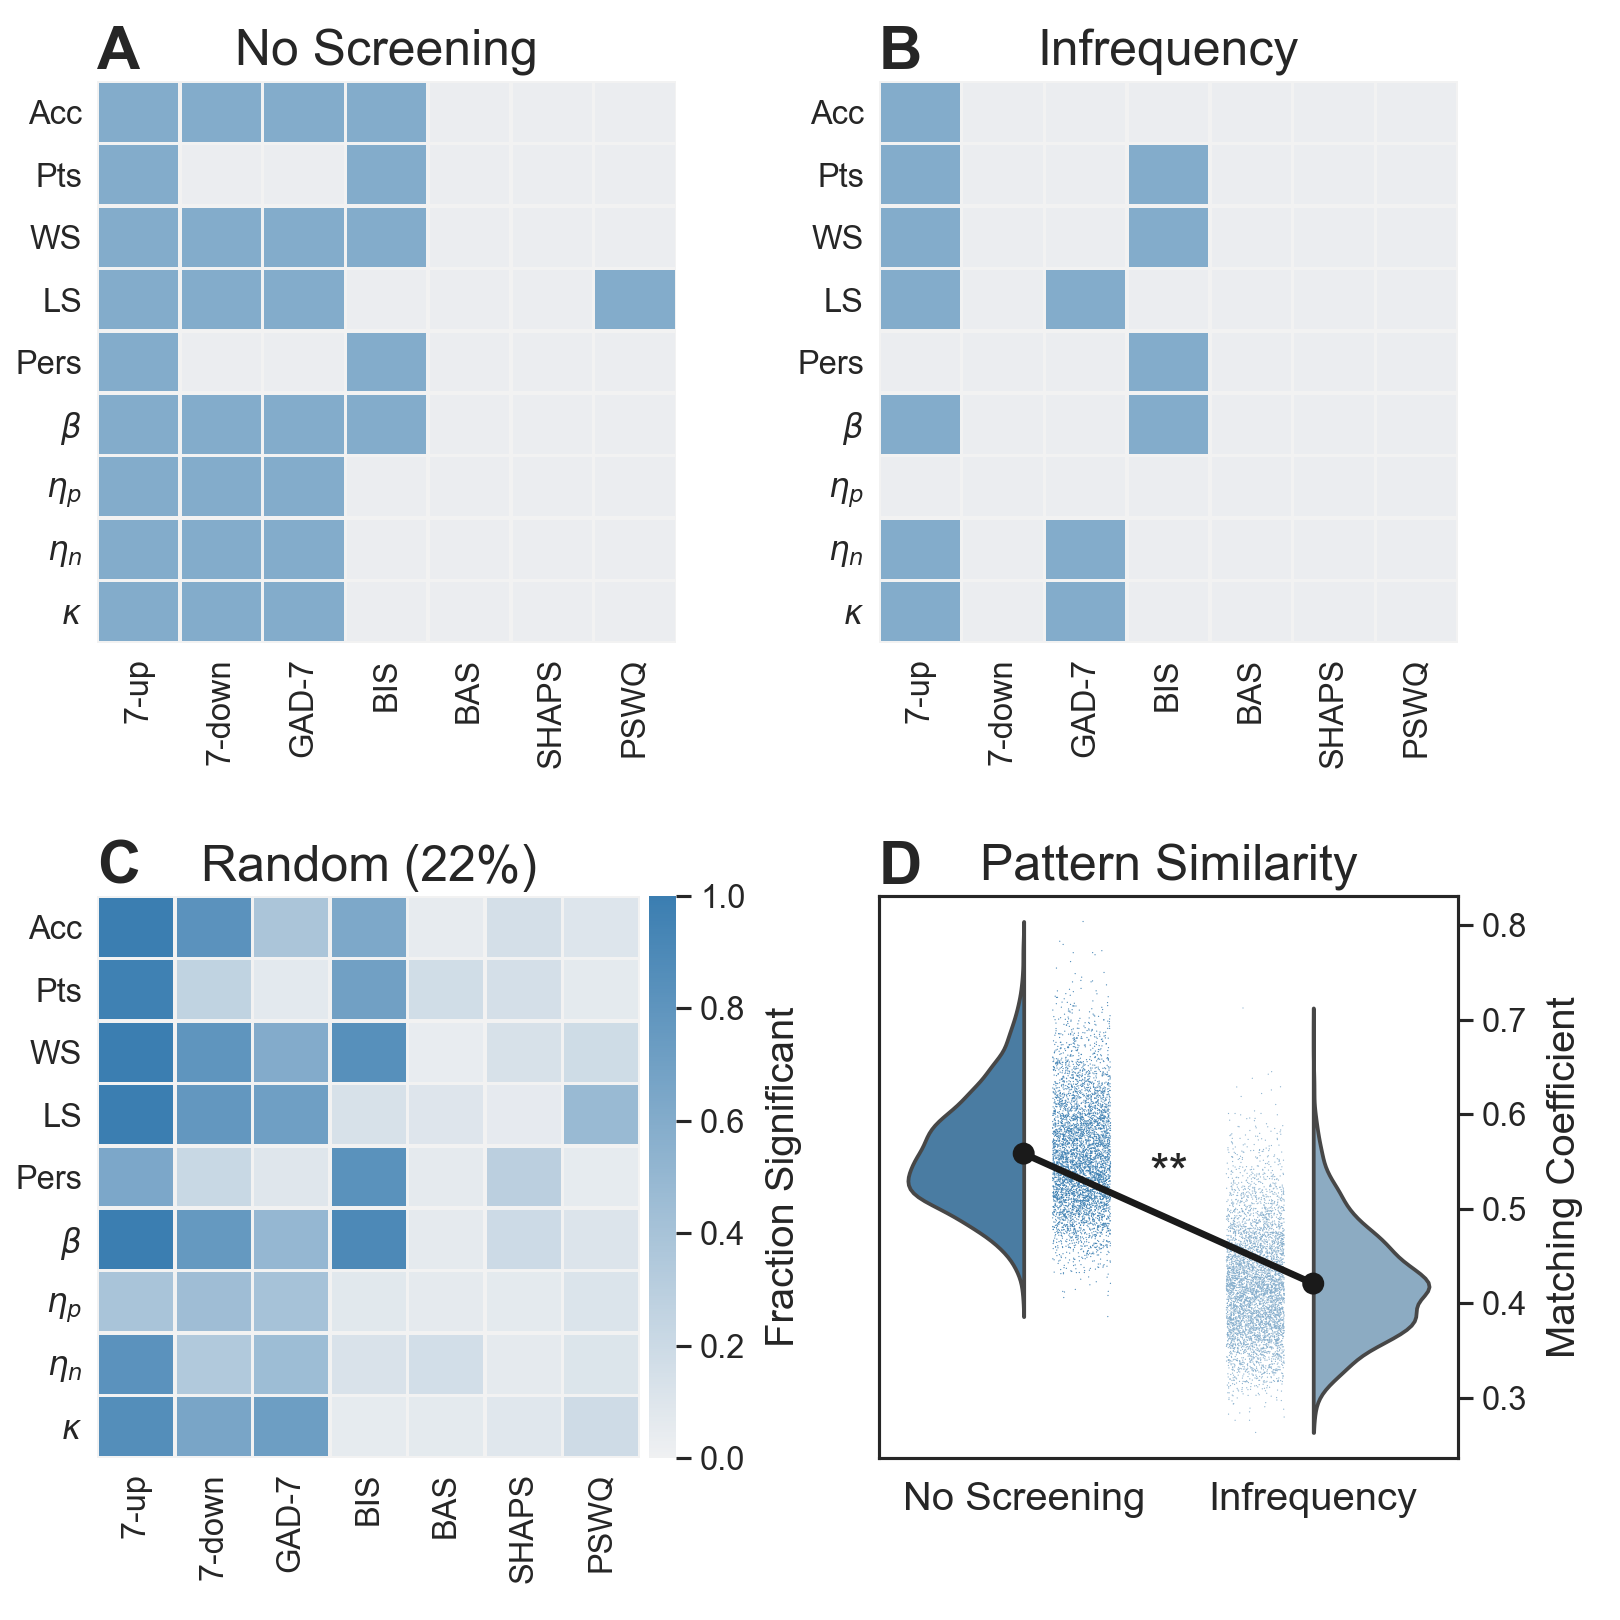
\includegraphics[width=17cm]{../figures/supp_01.png}
    \centering
    \caption{Signed Spearman rank correlations between task behavior (y-axis) and symptom measures (x-axis) under different regimes of data screening and participant exclusions. (A) No Screening = no exclusions ($N=386$). (B) Accuracy Only = exclusions based on chance-level performance in the reversal-learning task ($N=352$). (C) Infrequency Only = exclusions based on invalid or improbable responses to infrequency items ($N=301$). (D) Both Types = exclusions based on the previous two measures ($N=283$). Only statistically significant correlations are shown ($p<0.05$ not corrected for multiple comparisons). Black Xs indicate significant correlations ablated under screening. Acronyms: Acc = choice accuracy; Pts = total points earned; WS = win-stay rate; LS = lose-shift rate; Pers = perseveration errors; $\beta$ = inverse temperature; $\eta_p$ = positive learning rate; $\eta_n$ = negative learning rate; $\kappa$ = learning rate asymmetry.}
    \label{fig:figS01}
\end{figure}

\clearpage
\subsection*{Bootstrapping Analysis}
\begin{figure}[H]
    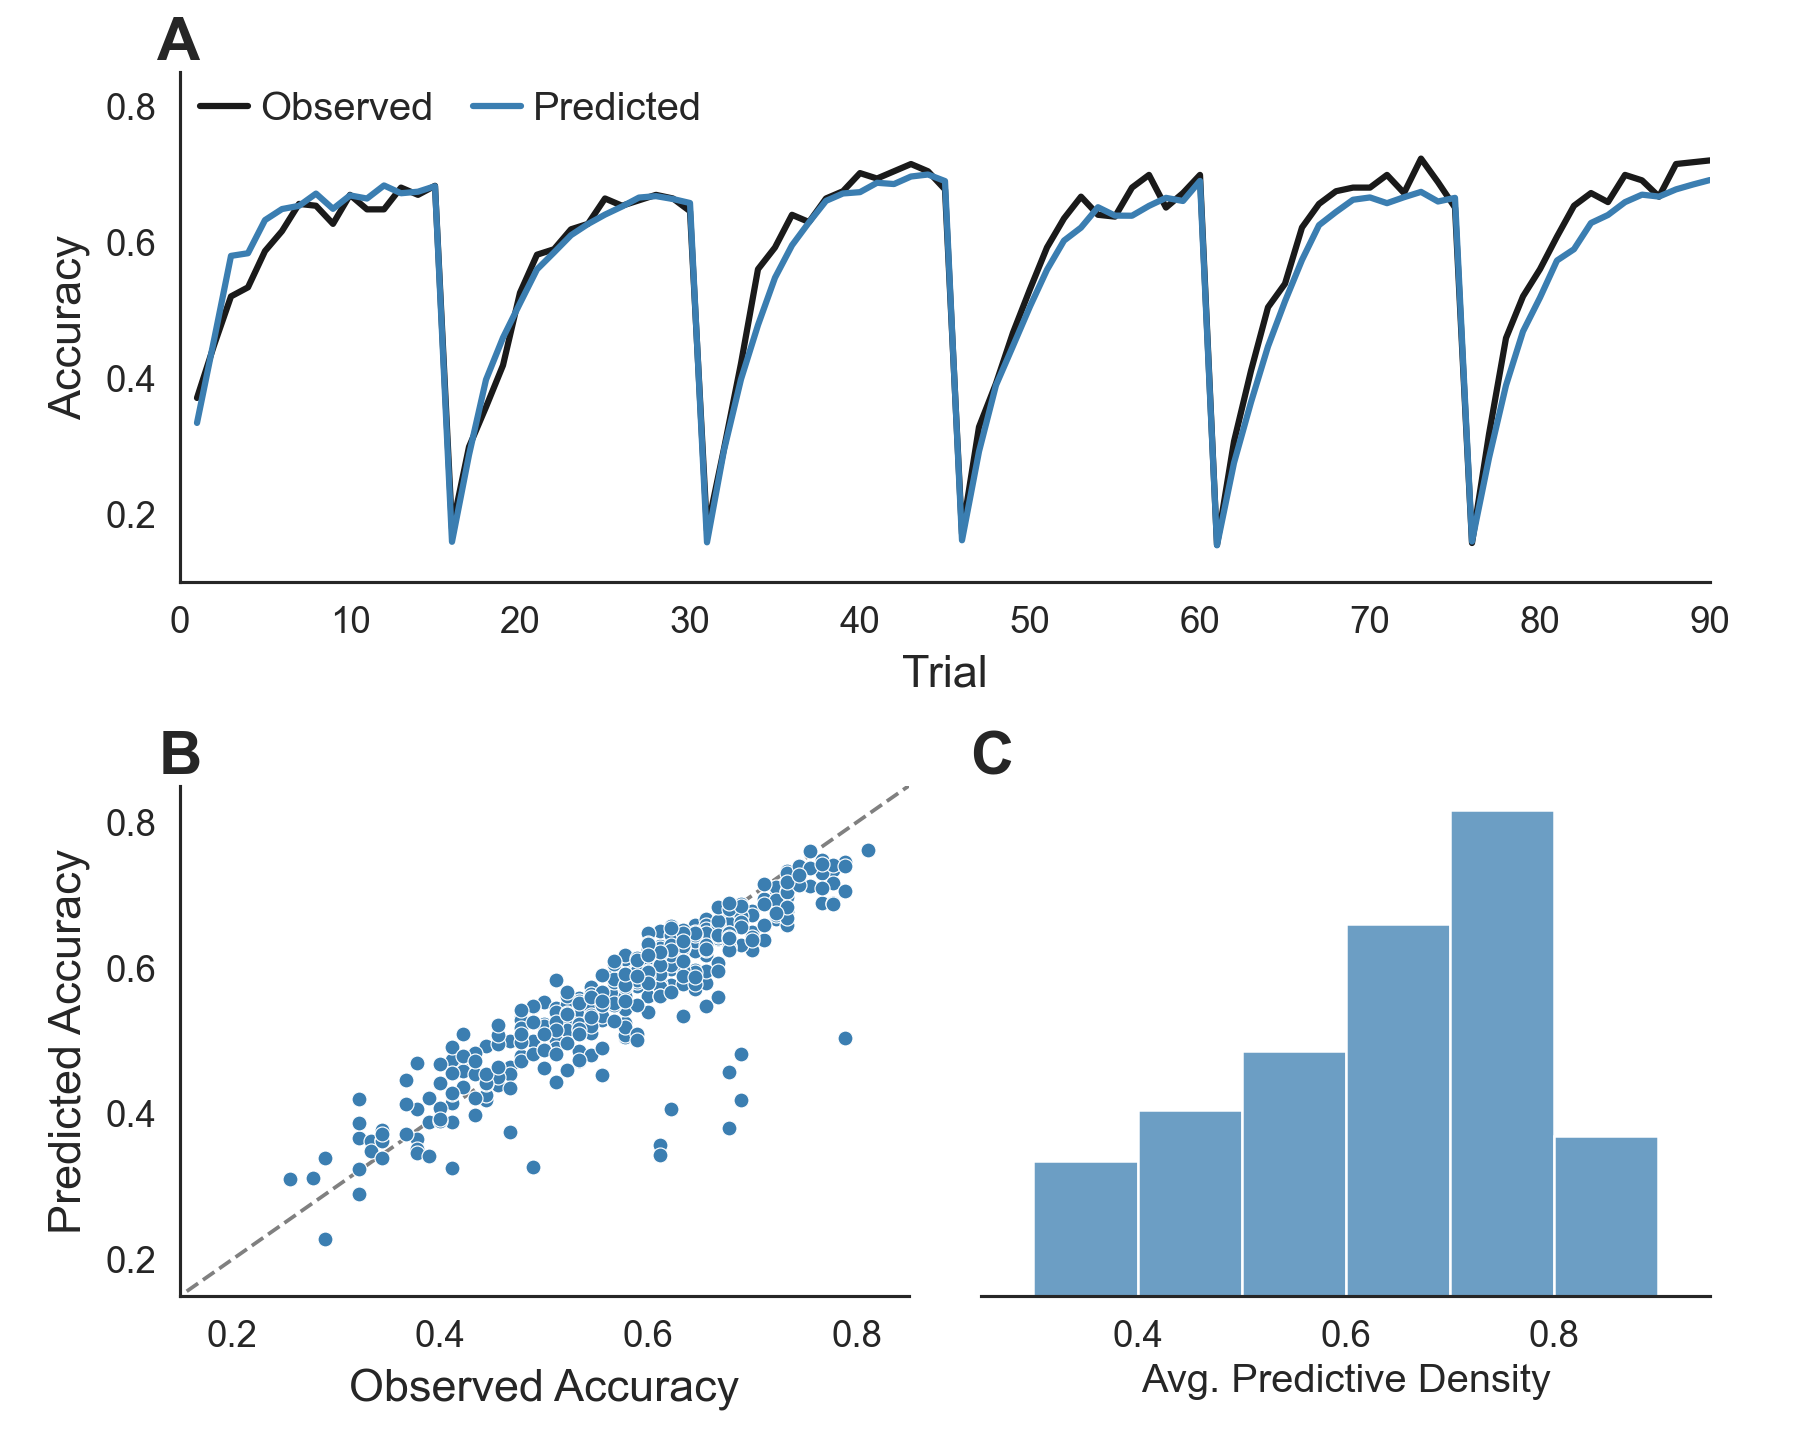
\includegraphics[width=16cm]{../figures/supp_02.png}
    \centering
    \caption{The pattern of significant behavior-symptom correlations before (A; $N=386$) and after (B; $N=301$) screening compared to the resulting pattern when random subsets of participants ($N=301$, matched to screening using the infrequency measure) are removed (C). Panels (A) and (B) are reproduced from Figure 4 for convenience. (C) The fraction of significant correlations in 5000 bootstrapped samples. (D) The similarity of the pattern of correlations after removal of random subsets to that before and after screening using the infrequency measure ($N=5000$ bootstrapped samples). Similarity was calculated using the simple matching coefficient. Random removal subsets were significantly more similar to the ``No Screening" than to the ``Infrequency" screening datasets (two-tailed, paired-samples $t$-test: $t = 262.490$, $p < 0.001$, $d = 3.713$, 95\% CI = [0.136, 0.138]).}
    \label{fig:figS02}
\end{figure}

\clearpage
\subsection*{The relationship between sample size and false positive rates generalize to other sets of variables}
\begin{figure}[H]
    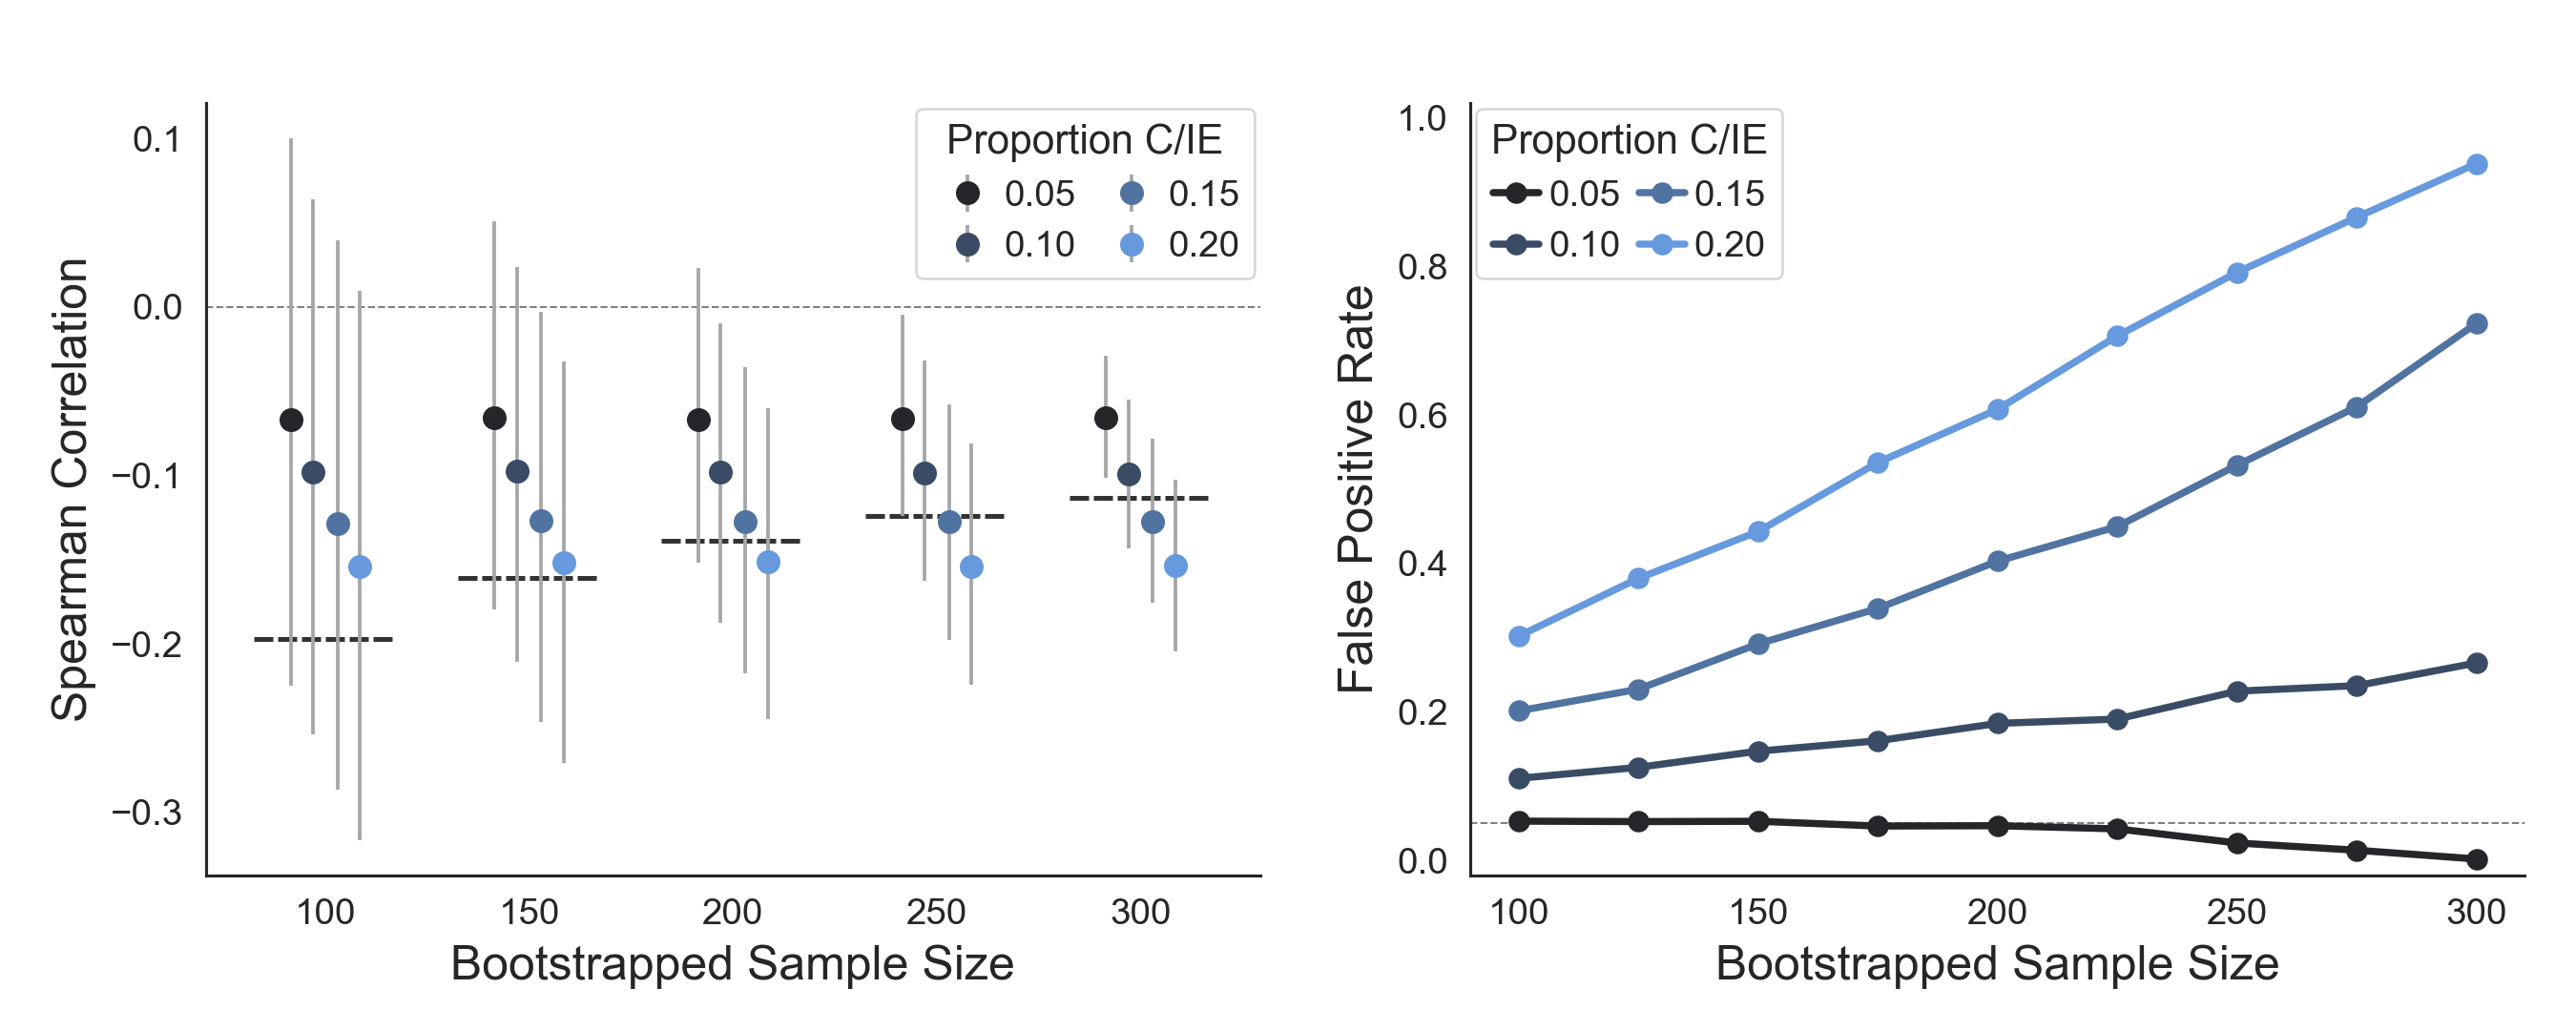
\includegraphics[width=16cm]{../figures/supp_03.png}
    \centering
    \caption{False positive rates for spurious correlations \emph{increase} with sample size. \textit{Left:} Spearman rank correlations and 95\% bootstrap confidence intervals between inverse temperature ($\beta$) and depression scores (7-down) as a function of sample size and proportion of C/IE participants. The thick dashed lines indicate the threshold for statistical significance for the Spearman correlation at the corresponding sample size. Markers are jittered along the x-axis for legibility. \textit{Right:} False positive rates for inverse temperature ($\beta$) and depression scores (7-down) as a function of sample size and proportion of C/IE participants. False positive rate was calculated as the proportion of bootstrap samples in which the correlation between $\beta$ and 7-down was statistically significant. The horizontal dotted line denotes the expected false positive rate at $\alpha = 0.05$.}
    \label{fig:figS03}
\end{figure}

\clearpage
\subsection*{The relationship between sample size and true positive rates for true correlations}
\begin{figure}[H]
    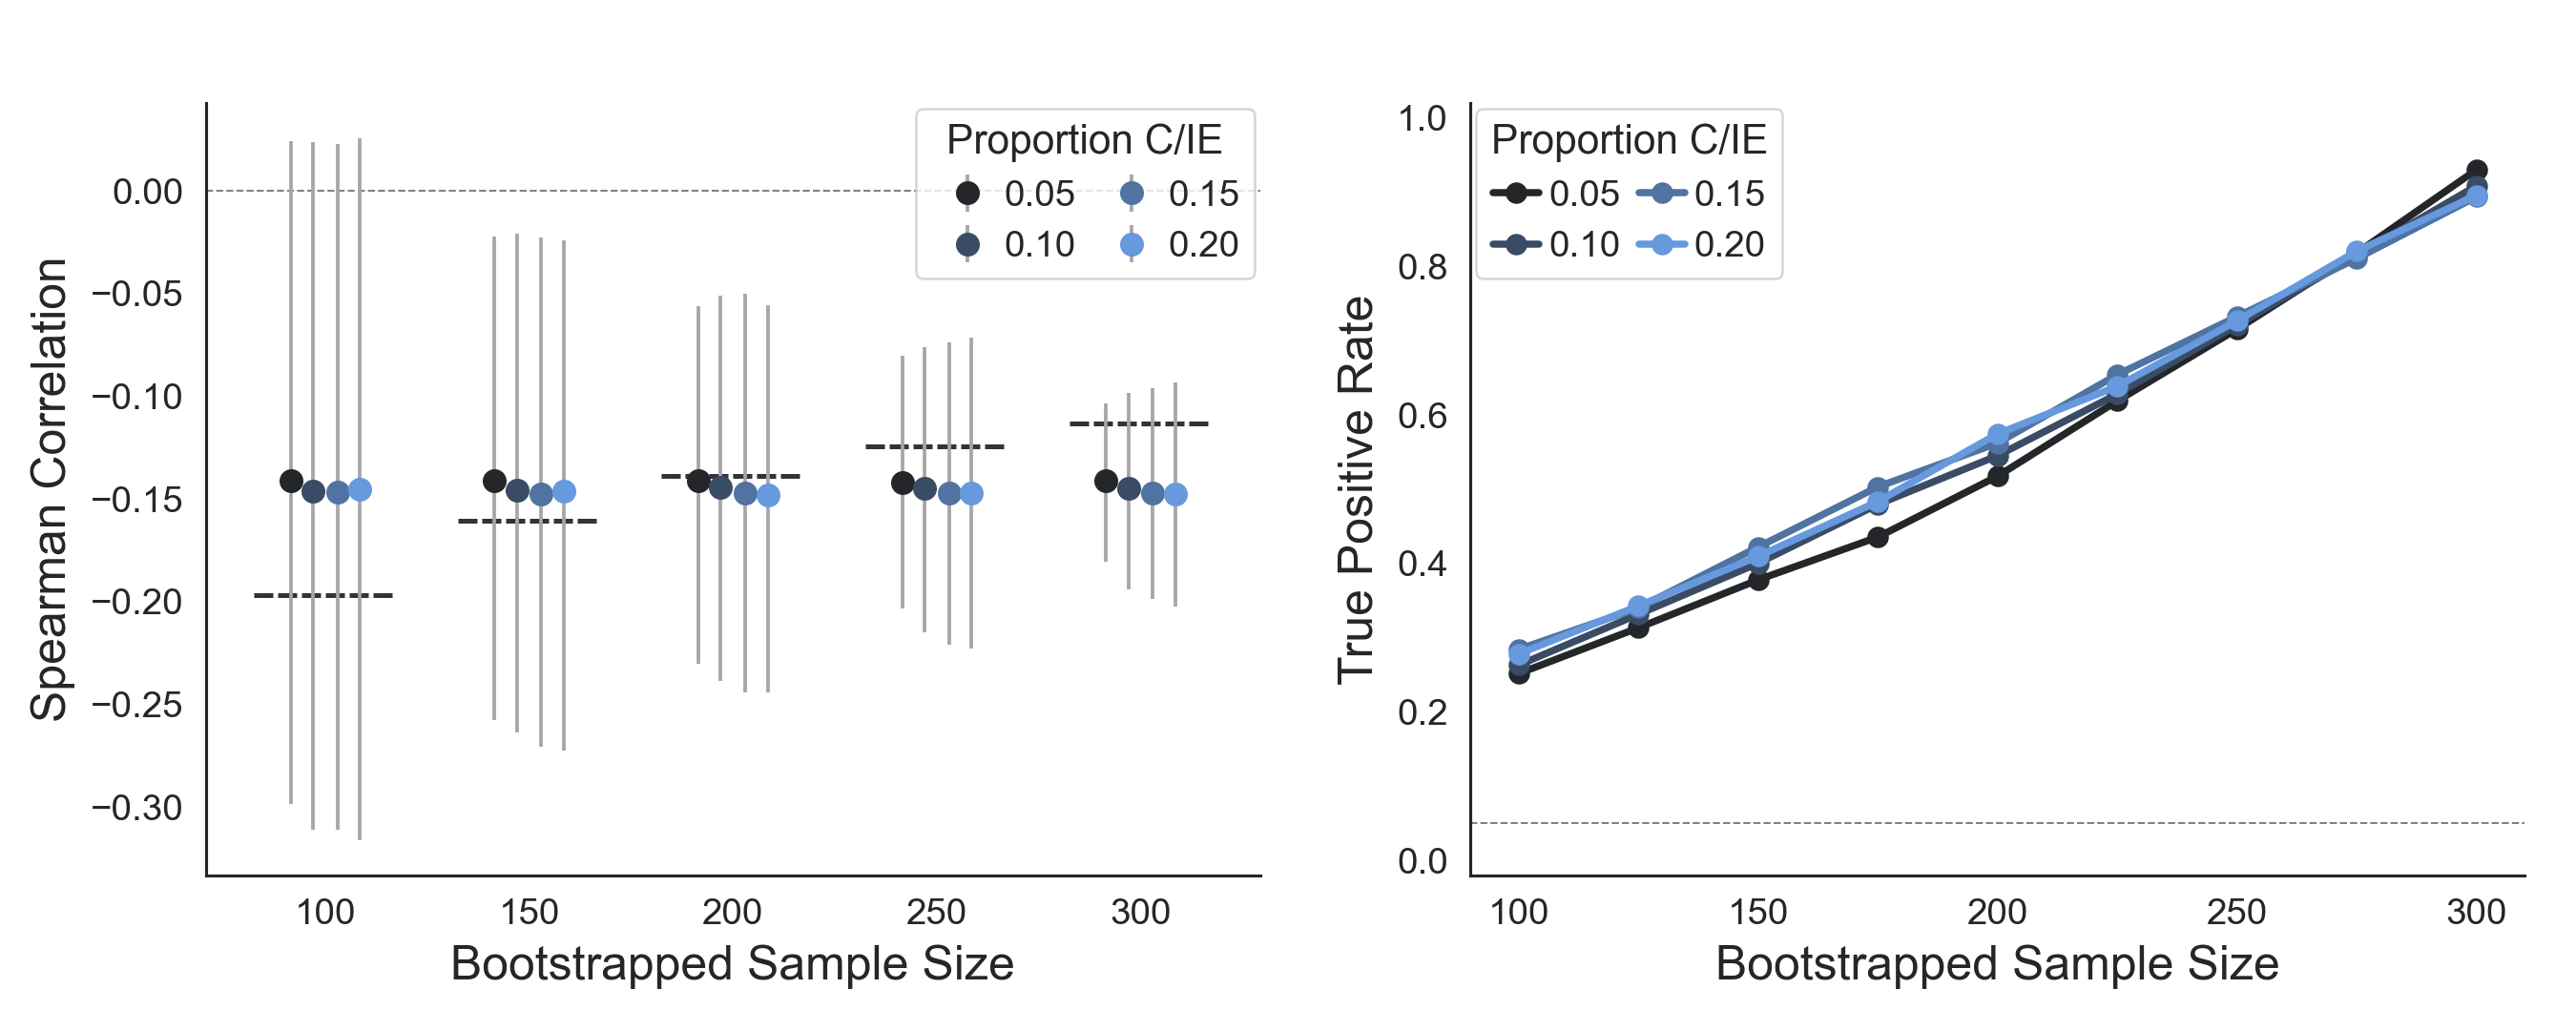
\includegraphics[width=16cm]{../figures/supp_04.png}
    \centering
    \caption{True correlations are independent of the proportion of C/IE participants in the sample. \textit{Left:} Spearman rank correlations and 95\% bootstrap confidence intervals between learning rate asymmetry ($\kappa$) and anxiety scores (GAD-7) as a function of sample size and proportion of C/IE participants. The thick dashed lines indicate the threshold for statistical significance for the Spearman correlation at the corresponding sample size. Markers are jittered along the x-axis for legibility. \textit{Right:} True positive rates for learning rate asymmetry ($\kappa$) and anxiety scores (GAD-7) as a function of sample size and proportion of C/IE participants. True positive rate was calculated as the proportion of bootstrap samples in which the correlation between $\kappa$ and GAD-7 was statistically significant. The horizontal dotted line denotes the expected false positive rate at $\alpha = 0.05$.}
    \label{fig:figS04}
\end{figure}

\clearpage

\subsection*{Posterior predictive checks}
\begin{figure}[H]
    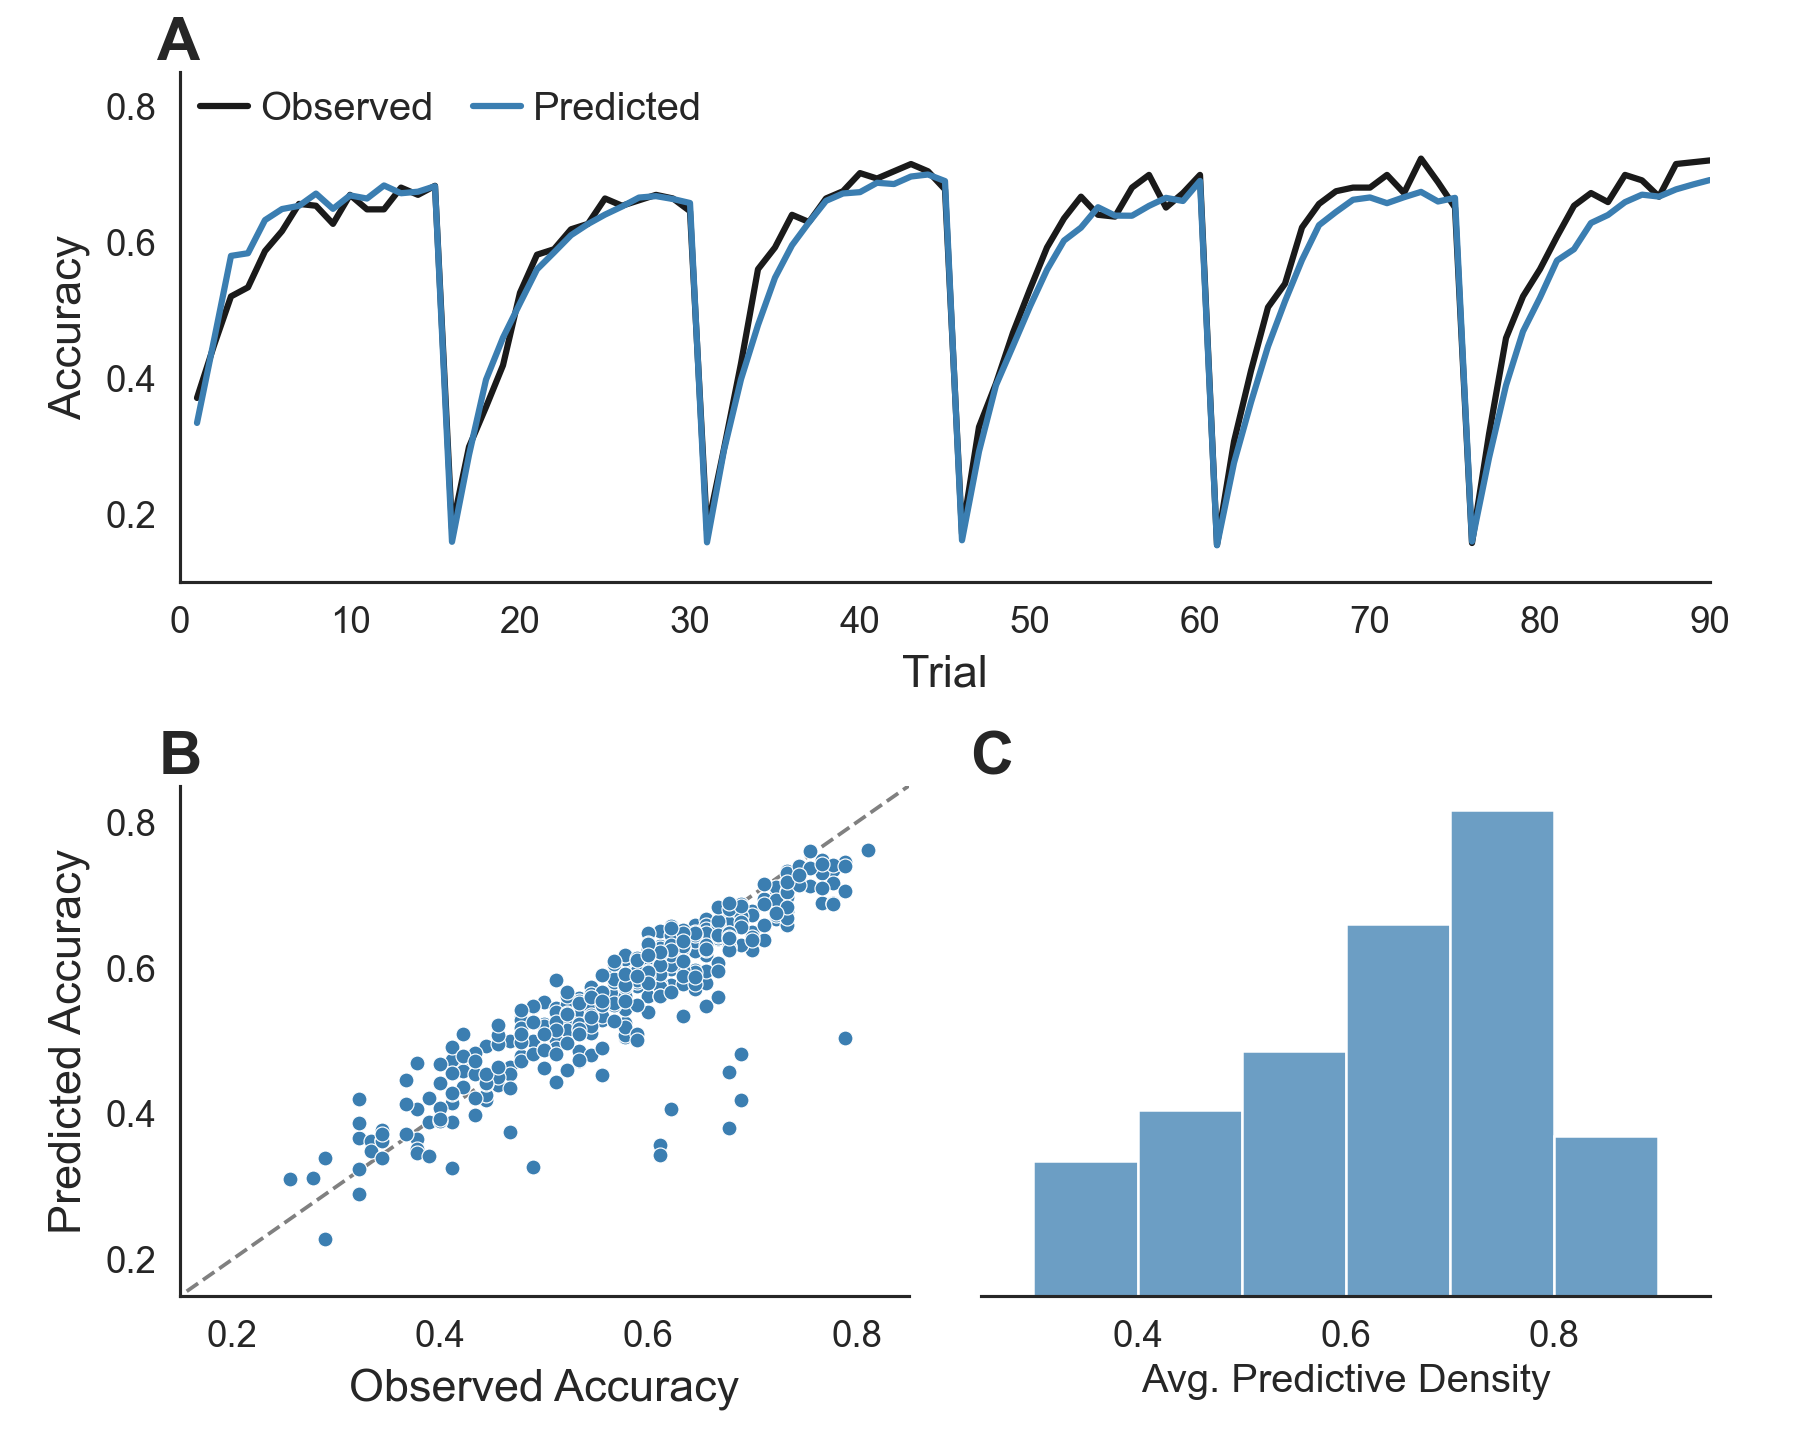
\includegraphics[width=16cm]{../figures/supp_05.png}
    \centering
    \caption{Posterior predictive checks for the risk-sensitive temporal difference learning model. (A) Observed (black) and predicted (blue) learning curves averaged across the group ($N=375$). (B) Observed versus predicted choice accuracy across participants ($N=375$). (C) Distribution of average predictive density across participants ($N=375$).}
    \label{fig:figS05}
\end{figure}

\clearpage
\subsection*{Participant demographics}
\begin{table}[!h]
    \centering
    \small
    \setlength{\tabcolsep}{15pt}
    \begin{tabular}{ rrrrr }
        \toprule
        & \multicolumn{2}{c}{MTurk} & \multicolumn{2}{c}{Prolific} \\
        \cmidrule(lr){2-3} \cmidrule(lr){4-5}
        Total & \multicolumn{2}{c}{N=186} & \multicolumn{2}{c}{N=200} \\
        \midrule
        Age & N & \% & N & \% \\
        \cmidrule(lr){1-5}
        18-25   &      16 &   8.6 &       78 &  39.0 \\
        26-35   &      76 &  40.9 &       69 &  34.5 \\
        36-45   &      46 &  24.7 &       31 &  15.5 \\
        46-55   &      22 &  11.8 &       13 &   6.5 \\
        55+     &      26 &  14.0 &        9 &   4.5 \\
        \midrule
        Gender & N & \% & N & \% \\
        \cmidrule(lr){1-5}
        Female             &    83 &  44.6 &    112 &  56.0 \\
        Male               &   103 &  55.4 &     85 &  42.5 \\
        Other              &     0 &   0.0 &      3 &   1.5 \\
        \midrule
        Ethnicity & N & \% & N & \% \\
        \cmidrule(lr){1-5}
        Hispanic or Latino     &    15 &   8.1 &     10 &   5.0 \\
        Not Hispanic or Latino &   168 &  90.3 &    183 &  91.5 \\
        Rather not say         &     2 &   1.1 &      7 &   3.5 \\
        Unknown                &     1 &   0.5 &      0 &   0.0 \\
        \midrule
        Race & N & \% & N & \% \\
        \cmidrule(lr){1-5}
        African American                 &    21 &  11.3 &      7 &   3.5 \\
        Asian                                     &     5 &   2.7 &     53 &  26.5 \\
        White                                     &   151 &  81.2 &    121 &  60.5 \\
        Multiracial                               &     6 &   3.2 &      4 &   2.0 \\
        Rather not say                            &     1 &   0.5 &     12 &   6.0 \\
        \midrule
        Use other platform & N & \% & N & \% \\
        \cmidrule(lr){1-5}
        Yes            &      71 &  38.2 &       28 &  14.0 \\
        No             &     115 &  61.8 &      172 &  86.0 \\
        \bottomrule
    \end{tabular}
    \caption{The demographics of each sample by online labor market. On average, the samples were similar though the sample from Mechanical Turk was older (two-tailed, two-sample $t$-test: $t(384)=6.567$, $p<0.001$, $d=0.669$, 95\% CI = [5.4, 10.0]) and comprised of fewer women (two-tailed, two-sample proportions test: $z(384)=2.529$, $p=0.011$, $h=0.258$, 95\% CI = [0.030, 0.228]). Note: the demographics do not include 20 participants excluded for participating in the study twice, once per platform.}
    \label{tab:tabS01}
\end{table}

\clearpage
\subsection*{Careless participants show different behaviors on the reversal learning task}
\begin{table}[H]
    \centering
    \begin{tabular}{lcccccc}
    \toprule
    {} &  Attentive &    C/IE &   $t$-value &   $p$-value &  Cohen's $D$ & 95\% CI \\
    \midrule
    Acc      &      0.587 &   0.532 &  4.008 &  $<$0.001 &  0.492 &    [0.028, 0.082] \\
    Pts      &     50.163 &  47.729 &  2.376 &     0.019 &  0.292 &    [0.426, 4.441] \\
    WS       &      0.898 &   0.776 &  5.387 &  $<$0.001 &  0.662 &    [0.077, 0.165] \\
    LS       &      0.609 &   0.751 & -5.335 &  $<$0.001 &  0.655 &  [-0.195, -0.090] \\
    Pers     &      0.245 &   0.259 & -1.505 &     0.139 &  0.185 &   [-0.033, 0.004] \\
    $\beta$  &      6.754 &   4.082 &  5.404 &  $<$0.001 &  0.664 &    [1.702, 3.640] \\
    $\eta_p$ &      0.643 &   0.551 &  2.846 &     0.007 &  0.350 &    [0.029, 0.157] \\
    $\eta_n$ &      0.738 &   0.784 & -1.516 &     0.120 &  0.186 &   [-0.106, 0.013] \\
    $\kappa$ &     -0.069 &  -0.218 &  3.729 &  $<$0.001 &  0.458 &    [0.071, 0.227] \\
    \bottomrule
    \end{tabular}
    \caption{Measures of task behavior compared between attentive ($N=301$) and C/IE ($N=85$) participants. Metrics compared using two-tailed, two-sample permutation $t$-tests ($df=384$, $\alpha = 0.05$, not corrected for multiple comparisons). Acronyms: Acc = choice accuracy; Pts = total points earned; WS = win-stay rate; LS = lose-shift rate; Pers = perseveration errors; $\beta$ = inverse temperature; $\eta_p$ = positive learning rate; $\eta_n$ = negative learning rate; $\kappa$ = learning rate asymmetry.}
    \label{tab:tabS02}
\end{table}

\clearpage
\subsection*{Correspondence of screening measures}

The following are the unthresholded results of the screening measure correspondence analyses.

\begin{table}[H]
    \centering
    \begin{adjustbox}{center}
    \tiny
    \begin{tabular}{rccccccccc}
        \toprule
        {} &      INF &      ISD &      REL &      MAH &    READ &     VAR &     ACC &   WSLS & RT \\
        \midrule
        INF  &                           - &                             &                             &                          &                 &                 &                            &                 &    \\
    ISD  &   \textbf{0.337 ($<$0.001)} &                           - &                             &                          &                 &                 &                            &                 &    \\
    REL  &  \textbf{-0.360 ($<$0.001)} &  \textbf{-0.804 ($<$0.001)} &                           - &                          &                 &                 &                            &                 &    \\
    MAH  &   \textbf{0.406 ($<$0.001)} &   \textbf{0.836 ($<$0.001)} &  \textbf{-0.608 ($<$0.001)} &                        - &                 &                 &                            &                 &    \\
    READ &              -0.111 (0.644) &   \textbf{0.209 ($<$0.001)} &     \textbf{-0.193 (0.002)} &            0.138 (0.220) &               - &                 &                            &                 &    \\
    VAR  &              -0.061 (1.000) &              -0.038 (1.000) &               0.068 (0.999) &           -0.024 (1.000) &  -0.026 (1.000) &               - &                            &                 &    \\
    ACC  &  \textbf{-0.206 ($<$0.001)} &              -0.133 (0.273) &               0.044 (1.000) &  \textbf{-0.182 (0.009)} &  -0.074 (0.996) &   0.027 (1.000) &                          - &                 &    \\
    WSLS &               0.060 (1.000) &               0.103 (0.794) &              -0.085 (0.971) &            0.115 (0.574) &   0.103 (0.790) &  -0.060 (1.000) &  \textbf{0.221 ($<$0.001)} &               - &    \\
    RT   &               0.040 (1.000) &              -0.025 (1.000) &               0.017 (1.000) &            0.013 (1.000) &  -0.158 (0.067) &  -0.007 (1.000) &             -0.094 (0.910) &  -0.050 (1.000) &  - \\
        \bottomrule
    \end{tabular}
    \end{adjustbox}
    \caption{Spearman rank correlations ($p$-value) of task and self-report data screening measures ($N=386$). Each entry corresponds to the Spearman correlation between two screening measures. Acronyms: INF = infrequency item; ISD = inter-item standard deviation; REL = personal reliability; MAH = Mahalanobis distance; READ = reading time; VAR = choice variability; ACC = choice accuracy; WSLS = win-stay lose-shift rate; RT = suspicious response times. Bolded entries indicate statistical significance for a two-sided rank correlation test ($\alpha = 0.05$, corrected for multiple comparisons).}
    \label{tab:tabS03}
\end{table}

\begin{table}[H]
    \centering
    \begin{adjustbox}{center}
    \tiny
    \begin{tabular}{rccccccccc}
        \toprule
        {} &     INF &     ISD &     REL &    MAH &   READ &    VAR &     ACC &  WSLS & RT \\
        \midrule
        INF  &                          - &                            &                            &                &                &                &                            &                &    \\
        ISD  &  \textbf{0.462 ($<$0.001)} &                          - &                            &                &                &                &                            &                &    \\
        REL  &  \textbf{0.484 ($<$0.001)} &  \textbf{0.691 ($<$0.001)} &                          - &                &                &                &                            &                &    \\
        MAH  &  \textbf{0.516 ($<$0.001)} &  \textbf{0.732 ($<$0.001)} &  \textbf{0.619 ($<$0.001)} &              - &                &                &                            &                &    \\
        READ &              0.319 (0.688) &              0.165 (1.000) &              0.165 (1.000) &  0.216 (1.000) &              - &                &                            &                &    \\
        VAR  &              0.208 (1.000) &              0.216 (1.000) &              0.238 (1.000) &  0.259 (1.000) &  0.292 (0.981) &              - &                            &                &    \\
        ACC  &     \textbf{0.379 (0.011)} &              0.312 (0.792) &              0.258 (1.000) &  0.344 (0.180) &  0.237 (1.000) &  0.282 (0.998) &                          - &                &    \\
        WSLS &              0.253 (1.000) &              0.247 (1.000) &              0.227 (1.000) &  0.258 (1.000) &  0.299 (0.964) &  0.303 (0.901) &  \textbf{0.505 ($<$0.001)} &              - &    \\
        RT   &              0.267 (1.000) &              0.219 (1.000) &              0.271 (1.000) &  0.271 (1.000) &  0.333 (0.363) &  0.251 (1.000) &              0.239 (1.000) &  0.260 (1.000) &  - \\
        \bottomrule
    \end{tabular}
    \end{adjustbox}
    \caption{Dice similarity coefficients ($p$-value) for task and self-report data screening measures for the top 10\% most suspicious participants. Each entry corresponds to the Dice coefficient between two screening measures for the 10\% most suspicious participants. Acronyms: INF = infrequency item; ISD = inter-item standard deviation; REL = personal reliability; MAH = Mahalanobis distance; READ = reading time; VAR = choice variability; ACC = choice accuracy; WSLS = win-stay lose-shift rate; RT = suspicious response times. Bolded entries indicate statistical significance for a two-sided Dice similarity permutation test ($\alpha = 0.05$, corrected for multiple comparisons).}
    \label{tab:tabS04}
\end{table}

\begin{table}[H]
    \centering
    \begin{adjustbox}{center}
    \tiny
    \begin{tabular}{rccccccccc}
        \toprule
        {} &     INF &     ISD &     REL &    MAH &    READ &    VAR &     ACC &   WSLS & RT \\
        \midrule
        INF  &                          - &                            &                            &                &                         &                &                            &                &    \\
        ISD  &  \textbf{0.355 ($<$0.001)} &                          - &                            &                &                         &                &                            &                &    \\
        REL  &  \textbf{0.355 ($<$0.001)} &  \textbf{0.564 ($<$0.001)} &                          - &                &                         &                &                            &                &    \\
        MAH  &  \textbf{0.355 ($<$0.001)} &  \textbf{0.667 ($<$0.001)} &  \textbf{0.359 ($<$0.001)} &              - &                         &                &                            &                &    \\
        READ &     \textbf{0.290 (0.006)} &              0.231 (0.231) &              0.154 (0.999) &  0.231 (0.231) &                       - &                &                            &                &    \\
        VAR  &              0.116 (1.000) &              0.080 (1.000) &              0.080 (1.000) &  0.160 (0.996) &           0.133 (1.000) &              - &                            &                &    \\
        ACC  &     \textbf{0.269 (0.020)} &              0.137 (1.000) &              0.164 (0.985) &  0.192 (0.809) &           0.247 (0.088) &  0.171 (0.968) &                          - &                &    \\
        WSLS &              0.242 (0.121) &              0.103 (1.000) &              0.154 (0.999) &  0.205 (0.635) &           0.231 (0.231) &  0.240 (0.140) &  \textbf{0.630 ($<$0.001)} &              - &    \\
        RT   &              0.164 (0.988) &              0.105 (1.000) &              0.132 (1.000) &  0.184 (0.879) &  \textbf{0.289 (0.007)} &  0.164 (0.985) &              0.225 (0.307) &  0.237 (0.162) &  - \\
        \bottomrule
    \end{tabular}
    \end{adjustbox}
    \caption{Dice similarity coefficients ($p$-value) for task and self-report data screening measures for the top 25\% most suspicious participants. Each entry corresponds to the Dice coefficient between two screening measures for the 25\% most suspicious participants. Acronyms: INF = infrequency item; ISD = inter-item standard deviation; REL = personal reliability; MAH = Mahalanobis distance; READ = reading time; VAR = choice variability; ACC = choice accuracy; WSLS = win-stay lose-shift rate; RT = suspicious response times. Bolded entries indicate statistical significance for a two-sided Dice similarity permutation test ($\alpha = 0.05$, corrected for multiple comparisons).}
    \label{tab:tabS05}
\end{table}

\clearpage
\subsection*{Correlations between behavior and symptom measures}

The following are the unthresholded results of the correlation analyses between task behavior and self-reported symptoms.  

\begin{table}[H]
    \centering
    \begin{adjustbox}{center}   
    \scriptsize
    \begin{tabular}{rccccccc}
        \toprule
        {} &       7u &       7d &    GAD-7 &      BIS &     BAS &   SHAPS &    PSWQ \\
        \midrule
        Acc      &  \textbf{-0.295 ($<$0.001)} &     \textbf{-0.166 (0.001)} &  \textbf{-0.093 (0.041)} &     \textbf{-0.134 (0.006)} &  -0.020 (0.328) &  -0.051 (0.158) &          -0.037 (0.232) \\
        Pts      &  \textbf{-0.225 ($<$0.001)} &              -0.076 (0.065) &           -0.023 (0.315) &     \textbf{-0.144 (0.003)} &  -0.061 (0.104) &  -0.051 (0.154) &           0.024 (0.321) \\
        WS       &  \textbf{-0.327 ($<$0.001)} &  \textbf{-0.160 ($<$0.001)} &  \textbf{-0.129 (0.009)} &  \textbf{-0.171 ($<$0.001)} &  -0.006 (0.449) &  -0.048 (0.178) &          -0.062 (0.116) \\
        LS       &   \textbf{0.285 ($<$0.001)} &   \textbf{0.158 ($<$0.001)} &   \textbf{0.146 (0.002)} &               0.050 (0.157) &  -0.037 (0.241) &   0.000 (0.494) &  \textbf{0.110 (0.015)} \\
        Pers     &      \textbf{0.134 (0.004)} &               0.066 (0.111) &            0.032 (0.271) &   \textbf{0.166 ($<$0.001)} &   0.018 (0.370) &   0.080 (0.064) &          -0.004 (0.469) \\
        $\beta$  &  \textbf{-0.370 ($<$0.001)} &  \textbf{-0.157 ($<$0.001)} &  \textbf{-0.114 (0.019)} &  \textbf{-0.185 ($<$0.001)} &   0.017 (0.377) &  -0.063 (0.105) &          -0.043 (0.204) \\
        $\eta_p$ &     \textbf{-0.097 (0.037)} &     \textbf{-0.105 (0.023)} &  \textbf{-0.101 (0.029)} &              -0.033 (0.274) &  -0.020 (0.351) &  -0.015 (0.402) &          -0.041 (0.213) \\
        $\eta_n$ &   \textbf{0.168 ($<$0.001)} &      \textbf{0.094 (0.032)} &   \textbf{0.108 (0.016)} &              -0.050 (0.165) &  -0.056 (0.143) &  -0.020 (0.351) &           0.042 (0.205) \\
        $\kappa$ &  \textbf{-0.175 ($<$0.001)} &     \textbf{-0.137 (0.004)} &  \textbf{-0.147 (0.002)} &              -0.008 (0.444) &  -0.020 (0.356) &  -0.028 (0.294) &          -0.061 (0.118) \\
        \bottomrule
    \end{tabular}
    \end{adjustbox}
    \caption{Spearman rank correlation ($p$-value) between task behavior and self-report symptom measures when no screening and rejections have been applied ($N=386$). Acronyms: Acc = choice accuracy; Pts = total points earned; WS = win-stay rate; LS = lose-shift rate; Pers = perseveration errors; $\beta$ = inverse temperature; $\eta_p$ = positive learning rate; $\eta_n$ = negative learning rate; $\kappa$ = learning rate asymmetry. Bolded entries indicate statistical significance for a two-sided rank correlation test ($\alpha = 0.05$, not corrected for multiple comparisons).}
    \label{tab:tabS06}
\end{table}

\begin{table}[H]
    \centering
    \begin{adjustbox}{center}
    \scriptsize
    \begin{tabular}{rccccccc}
        \toprule
        {} &       7u &       7d &    GAD-7 &      BIS &     BAS &   SHAPS &    PSWQ \\
        \midrule
        Acc      &  \textbf{-0.263 ($<$0.001)} &  \textbf{-0.144 (0.006)} &  \textbf{-0.105 (0.025)} &     \textbf{-0.106 (0.022)} &  -0.009 (0.436) &  -0.020 (0.363) &          -0.033 (0.272) \\
        Pts      &  \textbf{-0.187 ($<$0.001)} &           -0.042 (0.219) &           -0.020 (0.355) &     \textbf{-0.126 (0.009)} &  -0.055 (0.149) &  -0.028 (0.300) &           0.036 (0.254) \\
        WS       &  \textbf{-0.291 ($<$0.001)} &  \textbf{-0.137 (0.004)} &  \textbf{-0.123 (0.012)} &     \textbf{-0.161 (0.001)} &  -0.019 (0.358) &   0.006 (0.457) &          -0.044 (0.210) \\
        LS       &   \textbf{0.314 ($<$0.001)} &   \textbf{0.170 (0.001)} &   \textbf{0.156 (0.002)} &               0.034 (0.255) &  -0.036 (0.253) &  -0.037 (0.236) &  \textbf{0.124 (0.008)} \\
        Pers     &               0.083 (0.057) &            0.022 (0.348) &            0.011 (0.429) &      \textbf{0.151 (0.002)} &   0.010 (0.437) &   0.076 (0.090) &          -0.021 (0.338) \\
        $\beta$  &  \textbf{-0.332 ($<$0.001)} &  \textbf{-0.134 (0.004)} &  \textbf{-0.109 (0.027)} &  \textbf{-0.173 ($<$0.001)} &   0.010 (0.430) &  -0.040 (0.239) &          -0.023 (0.335) \\
        $\eta_p$ &              -0.056 (0.165) &           -0.089 (0.051) &  \textbf{-0.105 (0.024)} &              -0.013 (0.397) &  -0.029 (0.287) &   0.034 (0.271) &          -0.035 (0.265) \\
        $\eta_n$ &   \textbf{0.259 ($<$0.001)} &   \textbf{0.134 (0.004)} &   \textbf{0.122 (0.011)} &              -0.021 (0.351) &  -0.063 (0.130) &   0.019 (0.362) &           0.053 (0.161) \\
        $\kappa$ &     \textbf{-0.171 (0.001)} &  \textbf{-0.125 (0.008)} &  \textbf{-0.150 (0.002)} &              -0.016 (0.386) &  -0.032 (0.265) &  -0.033 (0.277) &          -0.060 (0.127) \\
        \bottomrule
    \end{tabular}
    \end{adjustbox}
    \caption{Spearman rank correlation ($p$-value) between task behavior and self-report symptom measures after applying rejections based on choice accuracy ($N=352$). Acronyms: Acc = choice accuracy; Pts = total points earned; WS = win-stay rate; LS = lose-shift rate; Pers = perseveration errors; $\beta$ = inverse temperature; $\eta_p$ = positive learning rate; $\eta_n$ = negative learning rate; $\kappa$ = learning rate asymmetry. Bolded entries indicate statistical significance for a two-sided rank correlation test ($\alpha = 0.05$, not corrected for multiple comparisons).}
    \label{tab:tabS07}
\end{table}

\begin{table}[H]
    \centering
    \begin{adjustbox}{center}        
    \scriptsize
    \begin{tabular}{rccccccc}
        \toprule
        {} &       7u &      7d &    GAD-7 &      BIS &     BAS &   SHAPS &    PSWQ \\
        \midrule
        Acc      &  \textbf{-0.210 ($<$0.001)} &  -0.048 (0.203) &            0.009 (0.433) &              -0.082 (0.078) &  -0.020 (0.360) &  -0.005 (0.454) &   0.009 (0.431) \\
        Pts      &     \textbf{-0.167 (0.001)} &   0.040 (0.234) &            0.070 (0.114) &     \textbf{-0.107 (0.030)} &  -0.046 (0.205) &  -0.011 (0.410) &   0.071 (0.114) \\
        WS       &  \textbf{-0.220 ($<$0.001)} &  -0.045 (0.226) &           -0.008 (0.450) &     \textbf{-0.143 (0.007)} &  -0.025 (0.322) &   0.001 (0.494) &   0.016 (0.386) \\
        LS       &   \textbf{0.219 ($<$0.001)} &   0.084 (0.069) &   \textbf{0.113 (0.026)} &               0.019 (0.364) &  -0.021 (0.351) &  -0.050 (0.186) &   0.082 (0.076) \\
        Pers     &               0.088 (0.068) &  -0.028 (0.312) &           -0.024 (0.347) &      \textbf{0.127 (0.015)} &   0.006 (0.457) &   0.048 (0.204) &  -0.052 (0.176) \\
        $\beta$  &  \textbf{-0.257 ($<$0.001)} &  -0.038 (0.254) &            0.047 (0.205) &  \textbf{-0.180 ($<$0.001)} &  -0.011 (0.428) &  -0.032 (0.301) &   0.056 (0.158) \\
        $\eta_p$ &              -0.052 (0.184) &  -0.064 (0.138) &           -0.079 (0.082) &              -0.015 (0.409) &  -0.008 (0.449) &   0.004 (0.474) &  -0.055 (0.173) \\
        $\eta_n$ &      \textbf{0.165 (0.002)} &   0.067 (0.120) &   \textbf{0.141 (0.007)} &              -0.037 (0.266) &  -0.089 (0.064) &  -0.030 (0.312) &   0.054 (0.174) \\
        $\kappa$ &     \textbf{-0.111 (0.029)} &  -0.046 (0.225) &  \textbf{-0.137 (0.008)} &               0.011 (0.426) &   0.015 (0.396) &   0.002 (0.484) &  -0.054 (0.180) \\
        \bottomrule
    \end{tabular}
    \end{adjustbox}
    \caption{Spearman rank correlation ($p$-value) between task behavior and self-report symptom measures after applying rejections based on infrequency items ($N=301$). Acronyms: Acc = choice accuracy; Pts = total points earned; WS = win-stay rate; LS = lose-shift rate; Pers = perseveration errors; $\beta$ = inverse temperature; $\eta_p$ = positive learning rate; $\eta_n$ = negative learning rate; $\kappa$ = learning rate asymmetry. Bolded entries indicate statistical significance for a two-sided rank correlation test ($\alpha = 0.05$, not corrected for multiple comparisons).}
    \label{tab:tabS08}
\end{table}

\begin{table}[H]
    \centering
    \begin{adjustbox}{center}        
    \scriptsize
    \begin{tabular}{rccccccc}
        \toprule
        {} &       7u &      7d &    GAD-7 &      BIS &     BAS &   SHAPS &    PSWQ \\
        \midrule
        Acc      &  \textbf{-0.229 ($<$0.001)} &  -0.090 (0.065) &           -0.072 (0.116) &           -0.053 (0.190) &   0.016 (0.383) &   0.034 (0.280) &  -0.040 (0.247) \\
        Pts      &     \textbf{-0.177 (0.003)} &   0.016 (0.388) &            0.011 (0.436) &           -0.086 (0.075) &  -0.013 (0.414) &   0.025 (0.324) &   0.038 (0.267) \\
        WS       &  \textbf{-0.227 ($<$0.001)} &  -0.085 (0.081) &           -0.057 (0.179) &  \textbf{-0.131 (0.016)} &  -0.025 (0.341) &   0.049 (0.201) &  -0.007 (0.461) \\
        LS       &   \textbf{0.236 ($<$0.001)} &   0.094 (0.059) &   \textbf{0.107 (0.036)} &            0.008 (0.453) &  -0.016 (0.387) &  -0.075 (0.101) &   0.079 (0.080) \\
        Pers     &               0.095 (0.056) &  -0.007 (0.459) &            0.014 (0.411) &   \textbf{0.110 (0.038)} &  -0.015 (0.392) &   0.037 (0.274) &  -0.025 (0.332) \\
        $\beta$  &  \textbf{-0.255 ($<$0.001)} &  -0.072 (0.121) &           -0.008 (0.457) &  \textbf{-0.165 (0.003)} &  -0.011 (0.426) &  -0.015 (0.405) &   0.028 (0.326) \\
        $\eta_p$ &              -0.045 (0.233) &  -0.088 (0.072) &  \textbf{-0.108 (0.029)} &            0.004 (0.473) &  -0.000 (0.505) &   0.049 (0.211) &  -0.073 (0.119) \\
        $\eta_n$ &   \textbf{0.196 ($<$0.001)} &   0.046 (0.213) &   \textbf{0.098 (0.047)} &           -0.015 (0.389) &  -0.085 (0.088) &   0.008 (0.459) &   0.024 (0.342) \\
        $\kappa$ &     \textbf{-0.114 (0.032)} &  -0.046 (0.228) &  \textbf{-0.134 (0.007)} &            0.007 (0.442) &   0.012 (0.425) &  -0.004 (0.495) &  -0.051 (0.209) \\
        \bottomrule
    \end{tabular}
    \end{adjustbox}
    \caption{Spearman rank correlation ($p$-value) between task behavior and self-report symptom measures after applying rejections based on both choice accuracy and infrequency items ($N=283$). Acronyms: Acc = choice accuracy; Pts = total points earned; WS = win-stay rate; LS = lose-shift rate; Pers = perseveration errors; $\beta$ = inverse temperature; $\eta_p$ = positive learning rate; $\eta_n$ = negative learning rate; $\kappa$ = learning rate asymmetry. Bolded entries indicate statistical significance for a two-sided rank correlation test ($\alpha = 0.05$, not corrected for multiple comparisons).}
    \label{tab:tabS09}
\end{table}

\clearpage
\subsection*{Task Instructions}

The following are the instructions given to participants for the probabilistic reversal learning task. As a reminder, the task was given a fishing-themed cover story. Each paragraph below denotes one screen of instructions.

\textit{Welcome to the fishing game! We will now give you some instructions on how to play the game. Use the buttons below (or the arrow keys) to navigate the instructions.}

\textit{In the fishing game, there are three beaches you can fish at. Each beach has its own unique surfboard. (The colors and pictures on the surfboards are there just to help you tell the beaches apart – they don’t have any special meaning other than that.)}

\textit{On each turn you will be shown three beaches, and you will choose which one you want to fish at. You can make your choice using the left, up, and right arrow keys.}

\textit{When you fish at a beach, you will either catch a fish or you will catch trash. Try to catch fish, and try not to catch trash!}

\textit{Some beaches are better than others. You are more likely to catch fish at some beaches (though you will still sometimes catch trash), and you are more likely to catch trash at other beaches (though you still sometimes catch fish).}

\textit{The beaches will change over time. As times goes by, you may be less likely to catch fish at a beach where you were previously catching many fish.}

\textit{Your goal is to catch as many fish as you can. You will receive a performance bonus up to \$0.25 that depends on how many fish you catch.}

\textit{Now we will ask you some questions about the game. You must answer all questions correctly to proceed. Feel free to read back through the instructions if there is anything you are not certain about.}

Following the instructions, participants completed a brief comprehension check where they were asked the following questions about the task:

\begin{enumerate}
    \item True or False: Your goal is to catch as many fish as you can. (True)
    \item True or False: You are more likely to catch fish at some beaches than others. (True)
    \item True or False: You will always catch fish at the best beach. (False)
    \item True or False: How likely you are to catch a fish at a beach stays the same over time. (False)
    \item True or False: The number of fish you catch will affect your final performance bonus. (True)
\end{enumerate}

Participants were required to answer all of the items correctly before they could proceed to the task. If they failed to do so, they restarted the instructions. There was no upper limit as to how many times a participant could loop through the instructions (the large majority of participants passed the comprehension check on their first try).

\subsection*{C/IE responding manifests as a distinct behavioral strategy}

In an exploratory analysis, we employed a theory-agnostic modeling approach to investigate how C/IE participants on the probabilistic reversal-learning task compared to attentive participants. The motivation for this analysis was to better understand why C/IE responding was inconsistently predicted by chance-level performance, and also correlated with asymmetric learning rates.  

To characterize participants' choice behavior, we adapted the softmax regression model from \cite{seymour2012serotonin}. This model estimates, for each participant, how much their choice depends on the recent history of trial events (rewarding outcomes, non-rewarding outcomes, and choices from the preceding 5 trials). Specifically, the influence of the history of particular type of event is defined as:

\begin{equation*}
    \sum_i^K w = x_{t-1} \cdot w_{t-1} + x_{t-2} \cdot w_{t-2} +  \ldots + x_{t-k} \cdot w_{t-k}
\end{equation*}

where $x_{t-i}$ is a binary indicator [0,1] denoting if an event (i.e., reward, non-reward, previous choice) occurred on trial $t-i$ and $w_{t-1}$ is the associated decision weight. These weights were estimated for rewards, non-rewards, and previous choices up to five trials in the past. The overall tendency to choose a particular choice option is dictated by a softmax choice rule:

\begin{equation*}
    p(y_t = i) = \frac{ \exp \left( \sum w_i^\text{reward} + \sum w_i^\text{nonreward} + \sum w_i^\text{choice} \right) }{ \sum_i \exp \left( \sum w_i^\text{reward} + \sum w_i^\text{nonreward} + \sum w_i^\text{choice} \right) }
\end{equation*}

Note that these weights were fit independently; that is, we did not employ an exponential kernel to parameterize the decay of the weights at successively distant trial lags. In sum then, the theory-agnostic model describes a participant's choice behavior as a function of 15 parameters. 

We fit the softmax regression model using Stan following the same procedure as for the theory-based analyses. Participant parameters were fit individually (i.e., not hierarchically)  so as to prevent bias during parameter estimation from partial-pooling between attentive and C/IE participants. Parameters were sampled with Gaussian priors with $\mu = 0$ and $\sigma = 5$.

The regression weights for each event, averaged within attentive and C/IE participants, are presented in Figure \ref{fig:regression}. Comparing attentive to C/IE participants, we observed a credible difference (i.e., 95\% highest density intervals excluded zero) only for the $T-1$ weight for previous choice. That is, attentive participants were more likely to repeat their previous choice (i.e., greater choice hysteresis) than were C/IE participants.

\begin{figure}[!t]
    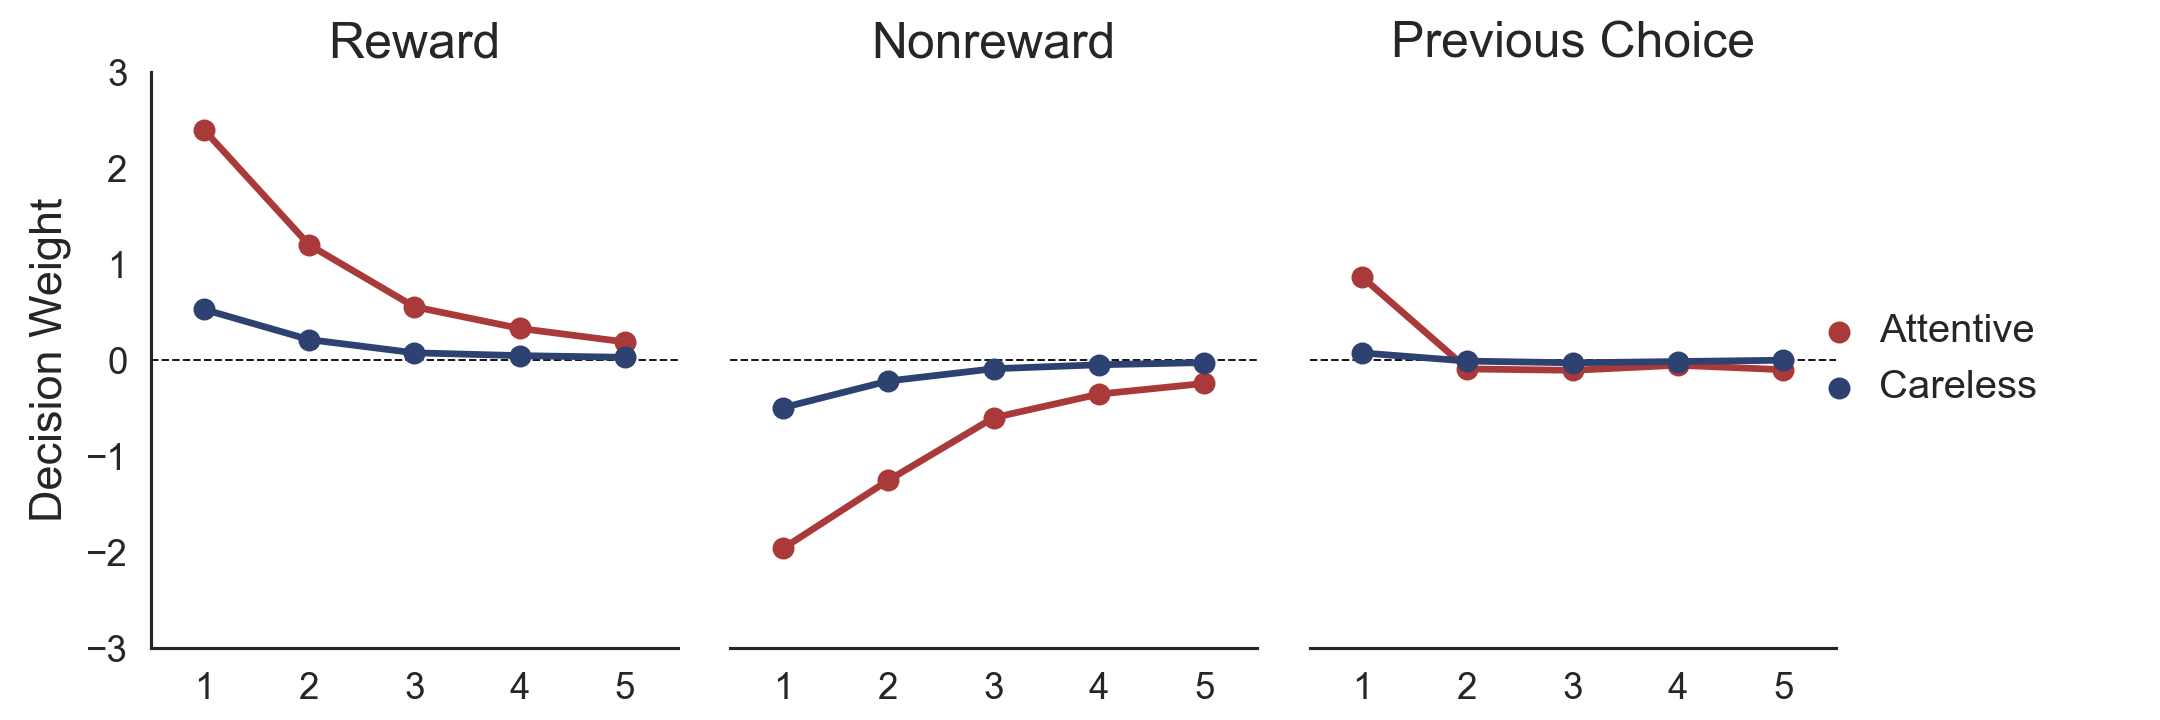
\includegraphics[width=16cm]{../figures/main_03c.png}
    \centering
    \caption{Softmax regression decision weights and 95\% highest density intervals in attentive (red) and C/IE (blue) participants. The weights reflect the extent to which the recent history of rewards, nonrewards, or previous choices influence current choice. *Denotes where the 95\% highest density interval of the difference in weights excluded zero.}
    \label{fig:regression}
\end{figure}

This result may be initially surprising, since one might expect choice hysteresis to result in more perseveration errors following contingency reversals. However, choice hysteresis is adaptive in this probabilistic reversal-learning task. Because rewards in the task are probabilistic, once the reward-maximizing response option has been identified ignoring an occasional unrewarding outcome and instead performing the same response is optimal (until the next reversal occurs and is identified). Interestingly, participants engaging in C/IE responding were also numerically (though not significantly) less affected by previous outcomes, suggesting that their behavior was not more adaptive, but rather just more random.

This pattern of results also helps explain the pre-screening correlations with asymmetric learning rates. Previous work has established that, when choice hysteresis is not accounted for in reinforcement learning models, it can manifest as positive learning rate asymmetries \cite{Katahira2018-ke, sugawara2021dissociation}. Since C/IE participants showed decreased hysteresis, which our reinforcement learning model did not explicitly account for, we should expect to find a negative correlation between learning-rate asymmetries and symptoms before C/IE participants are excluded. Indeed, this is what we observed above. 

In sum, the theory-agnostic analysis of task behavior revealed that C/IE participants exhibited a qualitatively distinct behavioral strategy on the probabilistic reversal-learning task. C/IE participants showed less adaptive choice hysteresis. Moreover, they were numerically (but not significantly) less sensitive to outcomes. The latter finding helps clarify in part why we observed low correspondence between task and self-report screening measures (that is, C/IE participants were not significantly more likely to respond randomly during the task). These results also present another hidden danger of C/IE responding: qualitatively distinct patterns of behavior under C/IE responding can bias the estimation of parameters of theoretical interest if not properly accounted for. 

\break
\section*{Appendix B: Replication study}

\subsection*{Background \& motivation}

Here we report a conceptual replication of our original study. The motivations for conducting a replication study were threefold. First, we wanted to examine the generalizability of our findings under new labor-platform conditions. Since summer 2020, when the original data were collected, online labor markets like Mechanical Turk/CloudResearch and Prolific Academic have undergone important changes. To address rampant data quality issues on Mechanical Turk, CloudResearch introduced their ``Approved Participants'' filter. When selected, only Mechanical Turk participants with a prior history of attentive and careful work are invited to participate in experiments \cite{cloudresearch_2020-2, hauser2021evaluating}. Similarly, a deluge of new, lower-quality users signed up to participate in studies on Prolific in summer, 2021 \cite{Letzter2021-bw}. In response, Prolific introduced new controls and filters to improve data quality on the platform \cite{prolific_2021}. In the wake of these changes, we wanted to explore the relevance of our original findings. Specifically, with these new safeguards, we wanted to examine whether the chance of spurious correlations has been considerably reduced. 

Second, we wanted to examine the generalizability of our findings to other behavioral measures. In the original study, we used a short, straightforward, and relatively easy reversal-learning task. Our motivation then was to demonstrate the risk of spurious correlations even for experiments where the possibility of participant fatigue (and consequently C/IE responding) had been minimized. One consequence of this design, however, was that the majority of participants performed reasonably well on the task (only 26 participants, or 7\% of the sample, exhibited choice accuracy at or below chance levels). This could in part explain why we observed such low correspondence between self-report and task-based screening measures. As such, we wanted to repeat our experiment and analyses using a more difficult task. Therefore, in the replication study we used the two-step task \cite{daw2011model}, which is both more challenging and takes longer than our original reversal-learning task. 

Finally, we wanted to examine the generalizability of our findings to other self-report measures. In the original study, we found that self-report symptom measures with low rates of endorsement were more likely to yield spurious correlations with behavior in the presence of C/IE responding, as C/IE participants were more likely to endorse symptoms, as well as to perform poorly on the task. In principle, this effect should not be limited to symptom measures, and should extend to any self-report measure with an expected skewed or asymmetric score distribution. Therefore, in the current replication study, we used two sets of self-report scales: one set of psychiatric symptom measures and one set of personality measures. As before, each set includes scales whose score distributions are expected to be symmetric as well as scales with asymmetric (skewed) score distributions. Crucially, the two personality scales we chose, artistic interests and greed avoidance, measure constructs that should have no meaningful relationship with model-based choice behavior on the two-step task. Therefore, the personality measures serve as a stronger test of our hypothesis that spurious correlations between self-report and behavioral measures are more likely for skewed score distributions. 

\subsection*{Methods}

\subsubsection*{Participants}

400 total participants were recruited to participate in an online behavioral experiment in February, 2022. Specifically, 200 participants were recruited from Amazon Mechanical Turk (MTurk) and 200 participants were recruited from Prolific. The study was approved by the Institutional Review Board of Princeton University (\#11968), and all participants provided informed consent. Total study duration was approximately 20 minutes. Participants received monetary compensation for their time (rate USD \$12/hr), plus an incentive-compatible bonus up to \$1.00 based on task performance. 

Participants were eligible if they resided in the United States or Canada. Participants from MTurk were recruited with the aid of CloudResearch services \cite{litman2017turkprime-2} using their ``Approved participants''  data quality filters \cite{cloudresearch_2020-2}. As in the original study, MTurk workers were not excluded based on work approval rate or number of previous jobs approved \cite{robinson2019tapped-2}. No other exclusion criteria were applied during recruitment.

Data from N=7 participants who completed the experiment were excluded prior to analysis because these participants (all from MTurk) disclosed that they had also completed the same experiment on the other platform. This left a final sample of N=393 participants (MTurk: N=193, Prolific: N=200) for analysis. The demographics of the sample split by labor market is provided in Table \ref{tab:S10}. Participants recruited from MTurk were older on average ($\Delta M = 4.9$ yrs; two-tailed, two-sample $t$-test: $t(391)=4.248$, $p<0.001$, $d = 0.429$, 95\% CI = [2.7, 7.2]) and comprised of fewer women (35.2\% versus 61\%; two-tailed, two-sample proportions test: $z(391)=5.500$, $p<0.001$, $h=0.562$, 95\% CI = [0.182, 0.372]). 

\begin{table}[!h]
    \centering
    \small
    \setlength{\tabcolsep}{15pt}
    \begin{tabular}{lrrrr}
        \toprule
        & \multicolumn{2}{c}{MTurk} & \multicolumn{2}{c}{Prolific} \\
        \cmidrule(lr){2-3} \cmidrule(lr){4-5}
        Total & \multicolumn{2}{c}{N=193} & \multicolumn{2}{c}{N=200} \\
        \midrule
        Age & N & \% & N & \% \\
        \cmidrule(lr){1-5}
        18-25   &    11 &   5.7 &     47 &  23.5 \\
        26-35   &    71 &  36.8 &     76 &  38.0 \\
        36-45   &    60 &  31.1 &     41 &  20.5 \\
        46-55   &    29 &  15.0 &     22 &  11.0 \\
        55+     &    22 &  11.4 &     14 &   7.0 \\
        \midrule
        Gender & N & \% & N & \% \\
        \cmidrule(lr){1-5}
        Female &      68 &  35.2 &      122 &  61.0 \\
        Male   &     124 &  64.2 &       73 &  36.5 \\
        Other  &       1 &   0.5 &        5 &   2.5 \\
        \midrule
        Ethnicity & N & \% & N & \% \\
        \cmidrule(lr){1-5}
        Hispanic or Latino     &    16 &   8.3 &     12 &   6.0 \\
        Not Hispanic or Latino &   177 &  91.7 &    180 &  90.0 \\
        Rather not say         &     0 &   0.0 &      8 &   4.0 \\
        \midrule
        Race & N & \% & N & \% \\
        \cmidrule(lr){1-5}
        American Indian/Alaska Native &     2 &   1.0 &      0 &   0.0 \\
        Asian                         &    15 &   7.8 &     41 &  20.5 \\
        Black or African American     &    13 &   6.7 &     12 &   6.0 \\
        White                         &   156 &  80.8 &    133 &  66.5 \\
        Multiracial                   &     6 &   3.1 &     10 &   5.0 \\
        Rather not say                &     1 &   0.5 &      4 &   2.0 \\
        \bottomrule
    \end{tabular}
    \caption{The demographics of each sample by online labor market.}
    \label{tab:S10}
\end{table}

\subsubsection*{Experiment}

Participants completed a gamified version of the two-step task \cite{daw2011model} designed to dissociate ``model-free'' and ``model-based'' decision-making. On every trial of the task, participants' goal is to collect as much ``space treasure'' as possible by traveling to one of two different planets and ``trading'' with one of two aliens who live on that planet. Participants first chose between two different-colored rocket ships (first-stage choice). Each rocket ship had a 70\% chance of traveling to one particular planet (e.g., the green rocket ship to the blue planet and the purple rocket ship to the red planet; common transitions) and a 30\% chance of traveling to the other planet (uncommon transition). The rocket ship and planet colors were randomized across participants, as were the mappings between rocket ships and planets. On each planet, participants chose which of two aliens to ``trade'' with (second-stage choice). If chosen, an alien would give the participant ``treasure'' with some slowly-changing probability, otherwise it would give ``junk''. The reward probabilities for each alien and trial were generated according to independent Gaussian random walks. Participants completed 201 trials of the task, with an optional break after the first half. 

Prior to the beginning of the experiment, participants had to read a set of instructions in which they were told that the rocket ships mostly traveled to one planet, but sometimes went to the other, and that the chance an alien would give them treasure would change slowly over the course of the task. Before they could start the task, participants had to correctly answer three sets of comprehension questions about the instructions. Failing to correctly answer all items forced the participant to reread a section of the instructions. Participants were permitted up to ten retries of the comprehension questions before they were removed from the experiment; however, no participant exceeded this limit. 

The task was programmed in jsPsych \cite{deleeuw_2015_jspsych-2} and distributed using custom web-application software. The experiment code is available at \url{https://github.com/nivlab/sciops}, and the web-software is available at \url{https://github.com/nivlab/nivturk}. A playable demo of the task is available at \url{https://nivlab.github.io/jspsych-demos/tasks/two-step/experiment.html}.

\subsubsection*{Self-report measures}

Prior to the start of the two-step task, participants completed four self-report measures in a randomized order. One was the 14-item seven-up/seven-down scale (7u/7d; \cite{youngstrom_2013_susd-2}), which measures lifetime incidence of depressive and (hypo)mania symptoms. This scale is expected to elicit lower rates of symptom endorsement, thereby resulting in asymmetric (right-skewed) score distributions. Participants also completed an alternative 7-item measure of general anxiety symptoms over the last year (e.g., ``I was overwhelmed by anxiety.''; \cite{watson2022development}). This scale is expected to elicit moderate rates of symptom endorsement, thereby resulting in a symmetric score distribution. We therefore expected the depression and mania measures to be at greater risk for spurious correlations with behavior on the two-step task than the anxiety measure. 

In addition, participants completed a 6-item measure of artistic interests (e.g., ``I believe in the importance of art''; \cite{ashton2007empirical}). Based on previous studies, this scale is expected to elicit high rates of endorsement, thereby resulting in an asymmetric score distribution. Finally, participants completed a 6-item measure of greed avoidance, which measures attitudes towards wealth and status (e.g., ``I am out for my own personal gain''; \cite{ashton2007empirical}). Based on previous studies, this scale is expected to elicit moderate rates of endorsement, thereby resulting in a symmetric score distribution. We therefore expected the artistic interests scale to be at greater risk for spurious correlations with behavior on the two-step task than the greed avoidance scale. 

\subsubsection*{Correspondence of screening measures}

As in the original study, we measured the correspondence of screening measures based on the task and self-report behavior. We calculated a number of standard measures of data quality from each participant's task behavior (four in total) and self-report responses (five in total). The self-report screening measures were identical to those used in the original study, except that we used (mostly) new infrequency items. We describe each of the new screening measures below.

\subparagraph{Self-report screening measure: Infrequency items.} Infrequency items are questions for which all (or virtually all) attentive participants should provide the same response. We embedded four infrequency items across the self-report measures. Specifically, we used the following questions:

\begin{enumerate}
  \item Have there been times in your life where you blinked your eyes at least once per day? (Expected response: \textit{Very often})
  \item Have there been times of a couple days or more when you were able to breathe underwater (without an oxygen tank)? (Expected response: \textit{Never or hardly ever})
  \item I was worried about the canine World Cup. (Expected response: \textit{Not at all})
  \item I have used a computer. (Expected response: \textit{Slightly Agree}, \textit{Agree}, or \textit{Strongly agree})
\end{enumerate}

Prior to conducting the study, the infrequency items were piloted on an independent sample of participants to ensure that they elicited one dominant response. We also included one instructed item (``Please select `Neutral' as your response'') to compare to the infrequency items. We measured the number of `suspicious' (i.e., incorrect) responses made by each participant to these questions. For thresholded analyses, participants were flagged if they responded incorrectly to one or more of these items. 

\subparagraph{Task-based screening variable: Side variability.} Side variability was defined as the fraction of trials a participant chose the left option (by pressing the left arrow key) across first stage choices during the two-step task. Side variability could range from 0.00 (only right arrow key used) to 1.00 (only left arrow key used). Extreme values (i.e., closer to zero or one) are indicative of more careless responding during the task, as the sides for which each choice option was displayed was determined randomly on each trial.  

\subparagraph{Task-based screening variable: Choice variability.} Choice variability was defined as the fraction of trials a participant chose the same first-stage choice option (randomized to the right or left side of the screen) during the two-step task. Choice variability could range from 0.00 (selected the green rocket ship exclusively) to 1.00 (selected the purple rocket ship exclusively). Extreme values (i.e., closer to zero or one) are indicative of more careless responding during the task as the most rewarding option changed throughout the task.  

\subparagraph{Task-based screening variable: Win-Stay Lose-Shift.} Win-stay lose-shift (WSLS) measures a participant's tendency to stay with a first-stage choice option following a second-stage reward versus shifting to a the other choice option following a non-reward. WSLS thus measures a participant's sensitivity to reward feedback. WSLS was estimated per participant via regression, predicting each first-stage choice (stay, switch) by the previous trial's outcome (reward, non-reward) and an intercept. We used the first (slope) term to represent a participant's WSLS tendency. Lower values of this term indicate less sensitivity to reward feedback and are thus indicative of more careless responding during the task. Thresholds for chance-level WSLS performance were determined by fitting the same regression model to 5000 randomly-generated datasets of first-stage choice (datasets were generated by matching the probability of staying with the previous trial's choice to the distribution observed empirically, but choices were otherwise independent across trials; that is, independent of previous outcome). The threshold for above-chance WSLS was defined as the 95th percentile of the distribution of slope estimates for the random data, corresponding to a one-tailed hypothesis test ($\alpha = 0.05$) that the slope coefficient is greater than zero. 

\subparagraph{Task-based screening variable: Response times.} ``Suspicious response time'' was defined as the proportion of first-stage choices with a response faster than 200ms. Greater proportions of outlier response times are indicative of more careless responding during the task.

\subparagraph{Correspondence Analysis.} We measured the correspondence of the above screening measures via two complementary approaches. First, we computed pairwise correlations on the unthresholded (continuous) measures using Spearman's rank correlation. Second, we estimated the pairwise rate of agreement on the binarized measures using the Dice similarity coefficient (looking at the top 10\% most suspicious respondents for each measure). The former approach estimates two measures' monotonic association, whereas the latter approach estimates their agreement as to which participants were most likely engaging in C/IE responding. For significance testing, we used permutation testing wherein a null distribution of similarity scores (Spearman's correlations or Dice coefficients) was generated for each pair of screening measures by iteratively permuting participants' identities within measures and re-estimating the similarity. P-values were computed by comparing the observed score to its respective null distribution. We corrected for multiple comparisons using family-wise error rates \cite{winkler2014permutation-2}.

\subsubsection*{Correlations between behavior and symptom measures}

To quantify the effects of both task and self-report data screening on behavior-symptom correlations, we estimated the pairwise correlations between the scale scores of each self-report measure and several measures of model-agnostic performance on the two-step task \cite{gillan2016characterizing}. Logistic regression analyses were conducted with the \textit{statsmodels} package \cite{seabold2010statsmodels} in the python programming language. The model tested if participants' first-stage choice behavior (coded as Stay = 1, Switch = 0) was influenced by the previous trial's reward (coded as Rewarded = 1, Unrewarded = 0), previous trial's transition (coded as Common = 1, Uncommon = 0), and their interaction. Importantly, the interaction term between previous reward and transition is a proxy for the contribution of model-based learning to choice behavior \cite{gillan2016characterizing}.

Correlations between the behavioral measures (i.e., logistic regression coefficients) and self-report measures were calculated using Spearman's rank correlation, after various forms of screening and exclusion. Significance testing was performed using the percentile bootstrap method \cite{wilcox2018guide-2} so as to avoid making any parametric assumptions. These correlation analyses were not corrected for multiple comparisons, since our overarching purpose was to demonstrate the extent of this issue across multiple behavioral measures and self-report symptoms. Any one of these correlations considered individually can be thought of as emulating a conventional analysis where fewer statistical tests would be performed.

\subsection*{Results}

\subsubsection*{Careless participants (often) appear symptomatic when the overall level of symptom endorsement is low}

To begin our analysis of the replication dataset, we examined the number of participants flagged by the WSLS and infrequency item screening measures. Only 31 participants (8\%) were flagged as exhibiting choice behavior at or below statistically chance levels in the two-step task. In contrast, 55 participants (14\%) endorsed a logically invalid or improbable response on one or more of the infrequency items when completing the self-report measures. The proportion of participants flagged for C/IE responding was significantly greater on Mechanical Turk compared to Prolific for both task (MTurk: N=23/193; Prolific: N=8/200; two-tailed, two-sample proportions test: $z(391)=2.911$, $p=0.004$, $h=0.305$, 95\% CI = [0.026, 0.132]) and survey data (MTurk: 34/193; Prolific: 21/200; two-tailed, two-sample proportions test: $z(391)= 2.033$, $p=0.042$, $h=0.206$, 95\% CI = [0.003, 0.140]). Across the four infrequency items, the average failure rate was 5.3\% (range: 2.5\% -- 8.9\%). In contrast, no participant failed the instructed item. This discrepancy in the proportion of participants flagged by each type of attention check is consistent with previous research, which found that instructed items are insensitive measures of C/IE responding \cite{barends2019noncompliant-2, thomas2017validity-2, hauser2016attentive-2}.   

\begin{figure}[t!]
    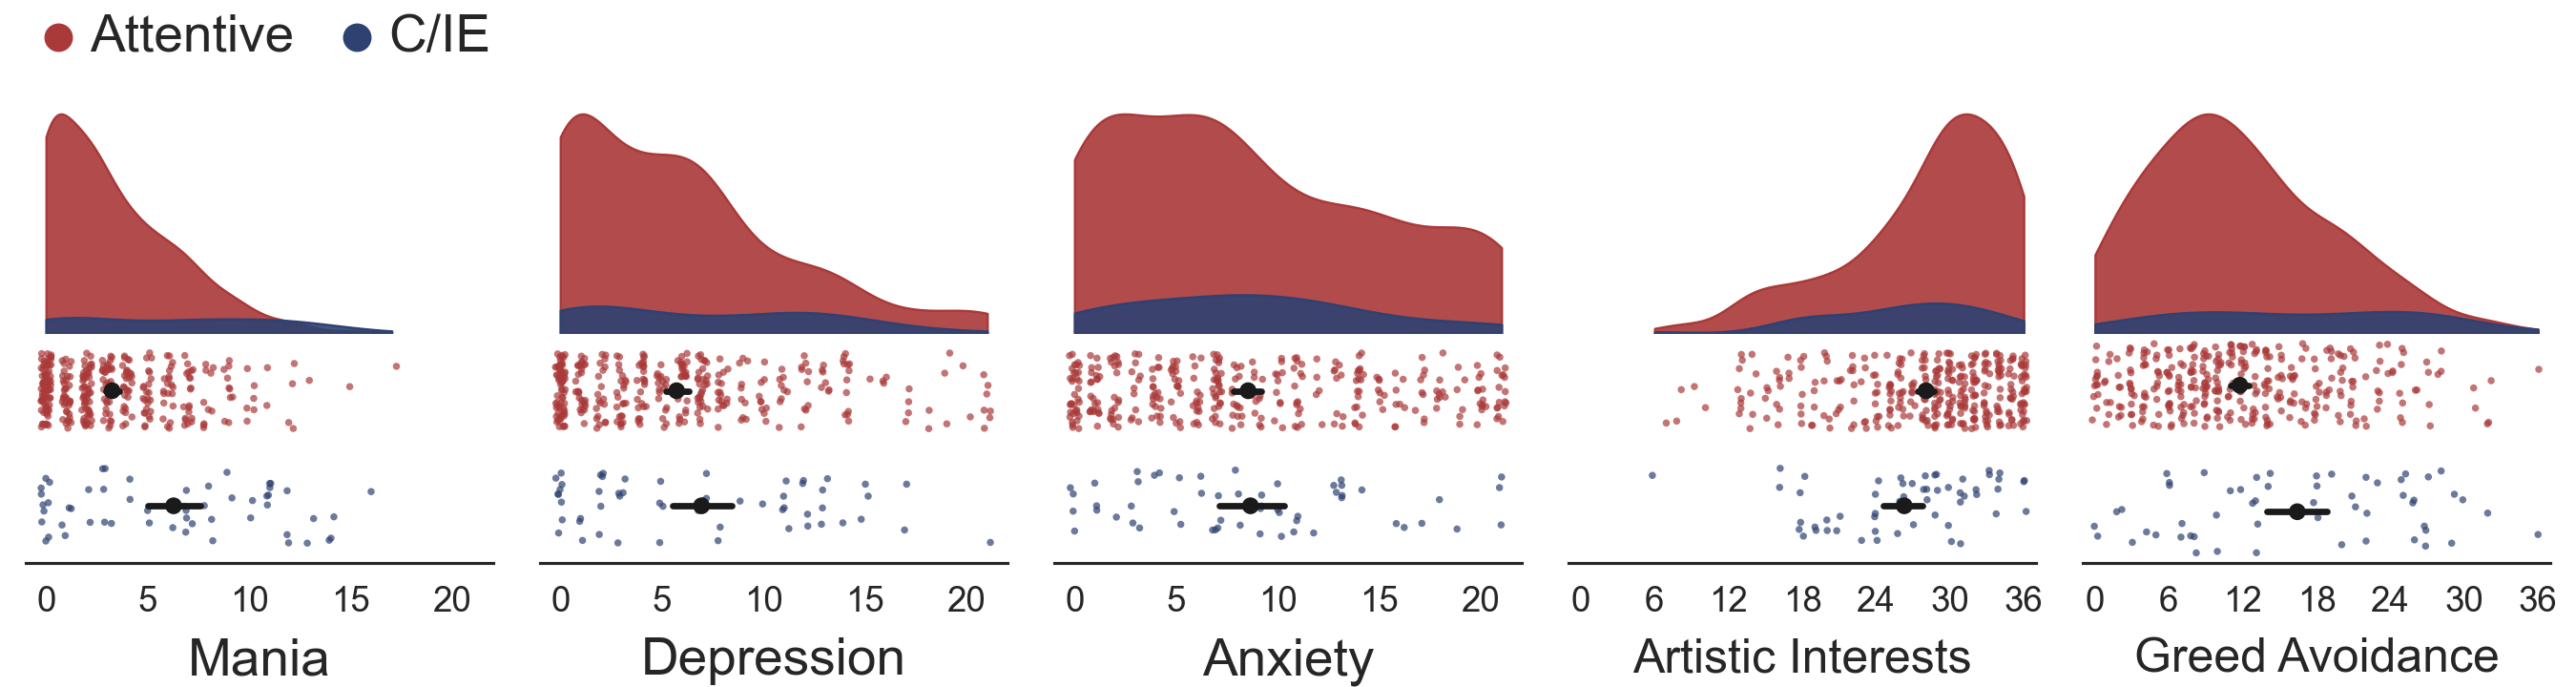
\includegraphics[width=15cm]{../figures/repl_02a.png}
    \centering
    \caption{Raincloud plots of total symptom scores in attentive ($N=338$; red) and C/IE ($N=55$; blue) participants. Each colored dot represents the symptom score for one participant. Black circles: average score within each group (error bars denote 95\% bootstrap confidence interval). Shaded plots: estimated distribution of responses for each group of participants.}
    \label{fig:S07}
\end{figure}

Previously, we observed a mean-shift in the average level of symptom endorsement for participants suspected of engaging in C/IE responding relative to attentive participants on measures for which the overall rate of symptom endorsement is low. This result was (mostly) replicated in the current dataset. Total scores were noticeably exaggerated in participants suspected of C/IE responding for the symptom measures where overall rates of symptom endorsement were the lowest (e.g., mania; Figure \ref{fig:S07}, leftmost plot). Where there were higher rates of symptom endorsement overall (e.g., anxiety), the distributions of symptom scores between the two groups of participants were more similar (Figure \ref{fig:S07}, middle plots). Permutation testing confirmed that observed mean-shifts in symptom scores for C/IE participants were statistically significant for the most skewed symptom measures (Table \ref{tab:S11}).

For the personality measures, however, an interesting pattern emerged (Figure \ref{fig:S07}, rightmost plots). We did not observe a statistically significant mean-shift in total scores for the subscale with the most skewed score distribution (i.e., artistic interests). However, an unexpected and statistically significant mean-shift in the average level of endorsement was observed for the more symmetrically-distributed greed-avoidance subscale. The reason for this finding is unclear. Regardless, this finding presents an opportunity to test for spurious correlations between behavioral and self-report measures in the presence of a mean-shift in scores in the absence of (substantially) skewed score distributions. 

\begin{table}[!t]
    \centering
    \small
    \begin{tabular}{lccccccc}
        \toprule
        Subscale & Skew &  Attentive & C/IE & $t$-value & $p$-value & Cohen's $D$ & 95\% CI \\
        \midrule
        Mania                &  1.065 &      3.249 &   6.273 & -6.054 &  $<$0.001 &  0.880 &  [-4.003, -2.045] \\
        Depression           &  0.889 &      5.719 &   6.945 & -1.572 &  0.119 &  0.229 &   [-2.756, 0.303] \\
        Anxiety              &  0.438 &      8.536 &   8.655 & -0.127 &  0.900 &  0.019 &   [-1.950, 1.712] \\
        Artistic interests   & -0.918 &     28.068 &  26.291 &  1.872 &  0.061 &  0.272 &   [-0.083, 3.637] \\
        Greed avoidance      &  0.550 &     11.769 &  16.436 & -4.166 &  $<$0.001 &  0.606 &  [-6.863, -2.472] \\
        \bottomrule
    \end{tabular}
    \caption{Comparison of the self-report total scores between attentive ($N=338$) and C/IE ($N=55$) participants. Scores compared using two-tailed, two-sample permutation $t$-test with $df=391$ ($\alpha = 0.05$, not corrected for multiple comparisons).}    
    \label{tab:S11}
\end{table}

\subsubsection*{Low correspondence between task and self-report measures of C/IE responding}

Next, we evaluated the degree of correspondence between behavioral and self-report screening measures to determine whether screening on behavior alone was sufficient to identify and remove careless participants. To measure the degree of correspondence between these behavioral and self-report screening measures, we performed two complementary analyses. First, we computed pairwise correlations on the unthresholded (continuous) measures using Spearman's rank correlation (Figure \ref{fig:S08}, left panel). After correcting for multiple comparisons, there were a handful of significant correlations between the behavioral and self-report screening measures. Abnormal response times emerged as the metric most correlated with the self-report screening measure. Crucially, as in the original study, the sizes of these observed correlations were roughly half those observed for the correlations between the self-report measures. 

\begin{figure}[!t]
    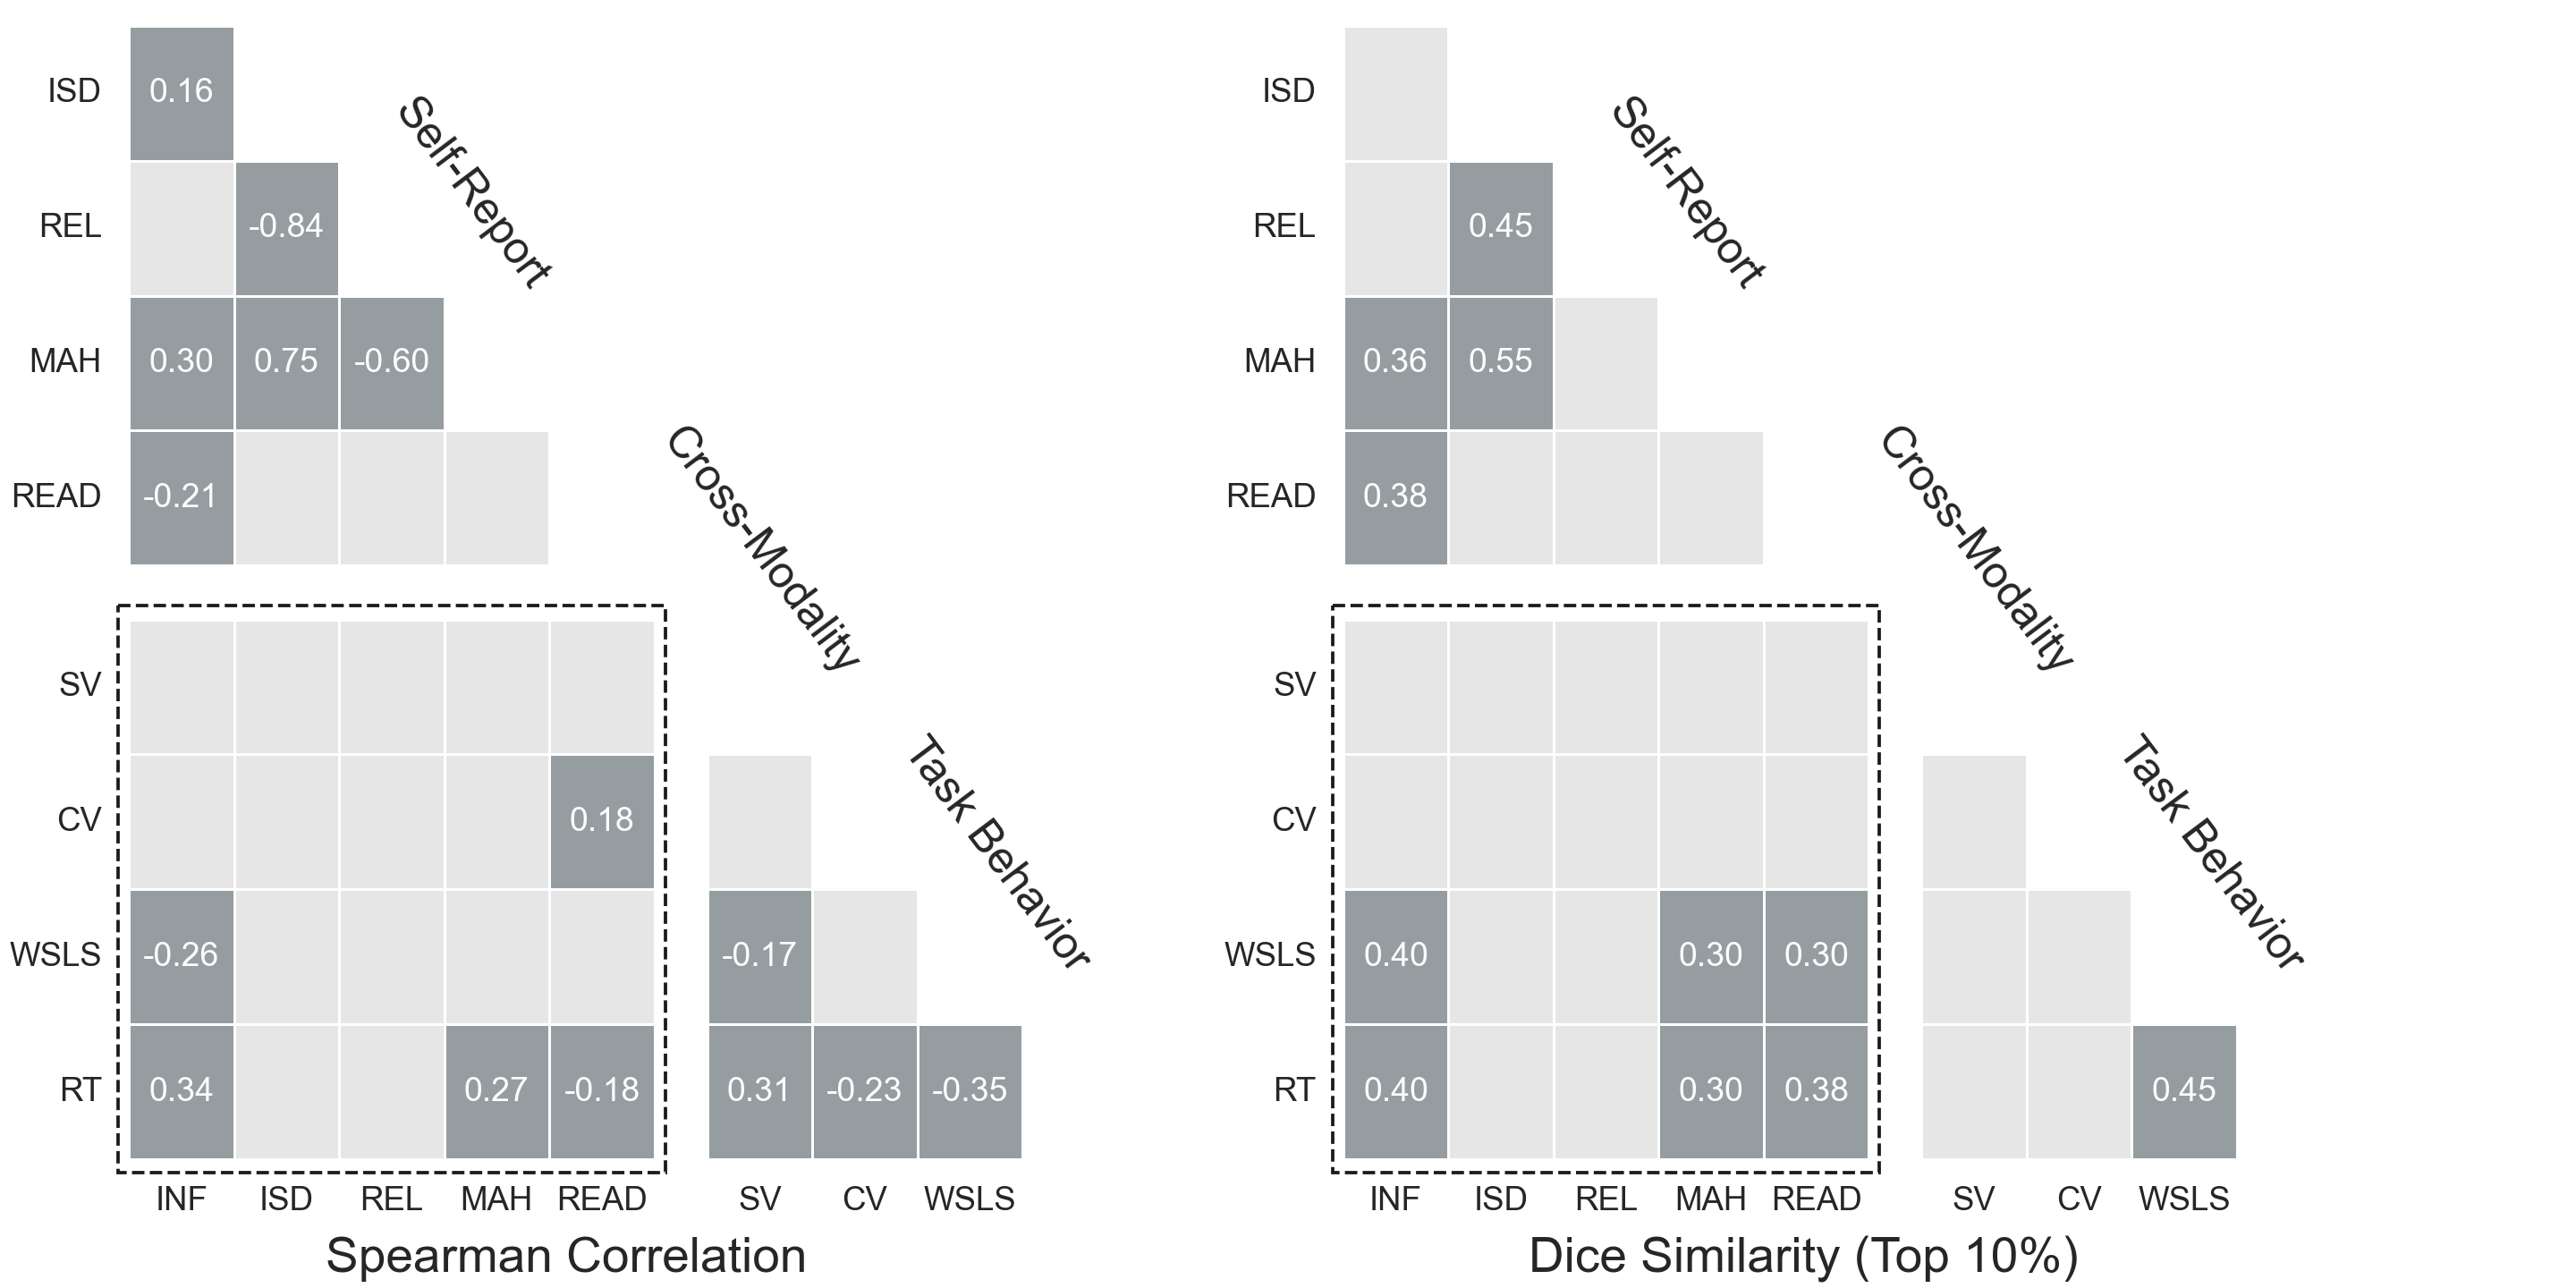
\includegraphics[width=16cm, trim=0 0 3cm 0]{../figures/repl_02b.png}
    \centering
    \caption{Similarity of task and self-report data screening measures. Each tile corresponds to the Spearman rank correlation (left) and Dice similarity coefficient (right) between two screening measures across $N=393$ participants. Acronyms: INF = infrequency item; ISD = inter-item standard deviation; REL = personal reliability; MAH = Mahalanobis distance; READ = reading time; SV = side variability; CV = choice variability; WSLS = win-stay lose-shift rate; RT = suspicious response times. Similarity scores have been thresholded after correcting for multiple comparisons. Numbers denote the strength of statistically significant correlations. Cross-modality correlations between task-behavior (left) and infrequency-item self-report measures (bottom) are in the dashed rectangle.}
    \label{fig:S08}
\end{figure}

Second, we used the Dice similarity coefficient to quantify agreement between different screening methods in the set of participants flagged for exclusion (Figure \ref{fig:S08}, right panel). This approach quantifies the degree of overlap between the set of would-be excluded participants based on different screening measures under a common exclusion rate. Results were largely consistent with the correlation analysis: only a handful of task and self-report screening measures achieved levels of agreement greater than what would be expected by chance. Of the significant cross-modality pairs, the average similarly coefficient was less than 0.4. In other words, when any of these sets of two measures are used to identify the top 10\% of participants most strongly suspected of C/IE responding, they agree on only two out of every five participants. Screening on task behavior alone would fail to identify the majority of participants most likely engaging in C/IE responding.

Taken together, these findings corroborate the results of the original study: measures of C/IE responding in task and self-report data do not identify the same set of participants. This means that solely excluding participants on the basis of poor behavioral performance---the most common approach in online studies---is unlikely to identify participants who engage in C/IE responding on self-report surveys. 

\subsubsection*{Spurious symptom-behavior correlations produced by C/IE responding}

To understand the effects of applying different forms of screening, we estimated the correlations between each unique pairing of a self-report measure and measure of behavior under four different conditions: no screening, screening only on task behavior (i.e., removing participants whose win-stay lose-shift behavior was not above chance), screening only on self-report responses (i.e., removing only participants who responded incorrectly on one or more infrequency items), or both. The resulting pairwise behavior-symptom correlations following each screening procedure are presented in Figure \ref{fig:S09}. We note that we did not correct these correlation analyses for multiple comparisons, since our purpose was to demonstrate the extent of this issue across multiple behavioral measures and self-report symptoms. Any one of these correlations considered individually can be thought of as emulating a conventional analysis where fewer statistical tests would be performed.

When no rejections were applied (i.e., all participants were included; Figure \ref{fig:S09}A), we observed multiple significant correlations between measures of task behavior and symptom scores for hypomania and depression. Consistent with our predictions, these correlations involved measures with low overall endorsement rates and mean-shifts in score distributions between attentive and C/IE participants. Conversely, we found no significant correlations with the symmetrically-distributed anxiety scores. This is despite the fact this scale measures symptoms that are comorbid with depression and mania. Crucially, of the two personality measures, we observed significant correlations only for the measure found to exhibit a mean-shift in scores between attentive and C/IE participants (i.e., greed avoidance). These included a significant correlation with the interaction term, which is used as a proxy measure for model-based choice behavior. That is, significant correlations were not restricted only to general behavioral measures but also to measures of specific theoretical interest.

Next, we excluded participants from the analysis based on task-behavior screening (i.e., lack of win-stay lose-shift behavior, removing the 8\% of participants exhibiting behavior indistinguishable from chance; Figure \ref{fig:S09}B). In contrast to the findings of the original study, the pattern of correlations was meaningfully changed: the putatively spurious correlations between greed avoidance and performance on the two-step task were ablated. Two previously significant correlations between hypomania and two-step performance were also rendered non-significant. A similar pattern of results was observed when we rejected participants based on self-report screening (removing 14\% of participants who endorsed one or more invalid or improbable responses on the infrequency items; Figure \ref{fig:S09}C) and when rejections were applied based on both task and self-report screening measures (removing 18\% of participants; Figure \ref{fig:S09}D).

\begin{figure}[!t]
    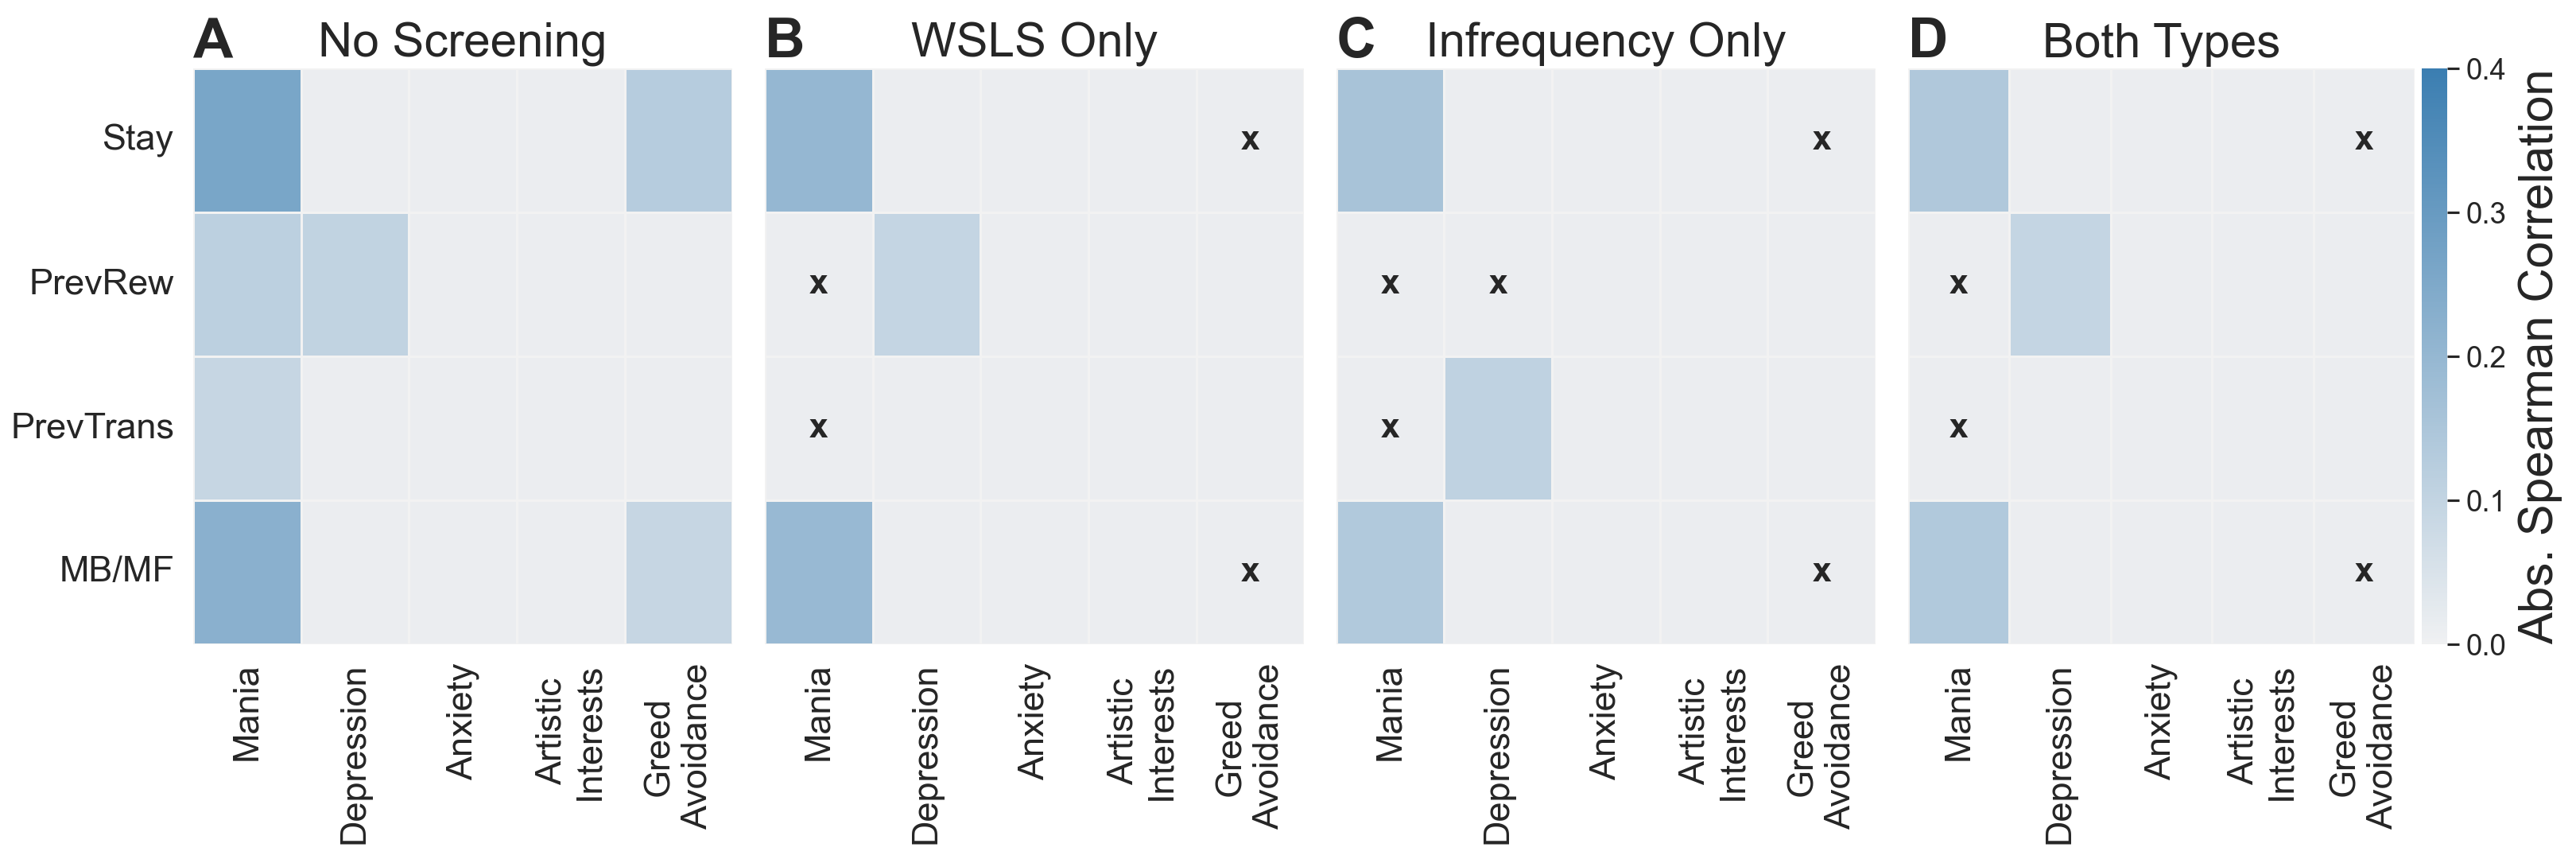
\includegraphics[width=17cm]{../figures/repl_03a.png}
    \centering
    \caption{Absolute Spearman rank correlations between task behavior (y-axis) and symptom measures (x-axis) under different regimes of data screening and participant exclusions. (A) No Screening = no exclusions. (B) WSLS Only = exclusions based on chance-level performance in the two-step task. (C) Infrequency Only = exclusions based on invalid or improbable responses to infrequency items. (D) Both Types = exclusions based on the previous two measures. Only statistically significant correlations are shown ($p<0.05$, not corrected for multiple comparisons). Black Xs indicate significant correlations ablated under screening. Acronyms: PrevRew = sensitivity to reward on the previous trial; PrevTrans = sensitivity to transition type on previous trial; MB/MF = index of model-based/model-free behavior (interaction between \textit{PrevRew} \& \textit{PrevTrans}).}
    \label{fig:S09}
\end{figure}

These findings suggest that some of the significant behavior-symptom correlations observed without strict participant screening may indeed be spurious correlations driven by C/IE responding. Interestingly, in contrast to the original study, with a more demanding behavioral task, screening based on either task behavior or self-report behavior alone was sufficient to protect against spurious symptom-behavior correlations in the presence of mean-shifts in scores between attentive and C/IE participants. For example, both forms of screening ablated the would-be significant correlation between model-based behavior and greed avoidance. The discrepancy in results between the original and replication studies may reflect the smaller numbers of participants failing attention checks in the replication study (14\%) compared to the original study (22\%), as well as differences in the behavioral tasks. Regardless, we replicate the findings of the original study in that screening on self-report data allowed us to identify symptom-behavior correlations most likely to be spurious.

\subsection*{Discussion}

Here we reported findings from a replication study whose purpose was to examine the generalizability of our original findings under new labor market conditions, different behavioral measures, and different self-report measures. To this end, we recruited an independent sample of almost 400 participants, using CloudResearch's and Prolific's latest data-quality filters, to complete the two-step task and a novel set of self-report measures. As evidence of the efficacy of the new data-quality filters, the proportion of participants flagged for C/IE responding in the self-report measures was noticeably smaller in the replication sample (14\%) compared to original sample (22\%). This decrease in the number of participants suspected of C/IE responding was observed for both MTurk and Prolific (though, as in the original study, the proportion of low-quality participants was significantly, albeit marginally, smaller for Prolific than MTurk). Regardless, although the new online labor platform quality-control measures seem to be effective, they did not completely solve the problem; indeed, the proportion of participants engaging in C/IE responding was reduced only by one-third.

Next, we compared the distribution of self-report scale scores for attentive participants and participants suspected of engaging in C/IE responding. Replicating our previous result, we observed a mean-shift in the average level of symptom endorsement for participants suspected of C/IE responding relative to attentive participants, only when the overall rate of symptom endorsement was low. Specifically, flagged participants showed significantly elevated scores on the hypomania scale (with its right-skewed score distribution) but not so on the anxiety scale (with its symmetric score distribution). Interestingly, we found the opposite pattern for the personality measures: scores for participants engaging in C/IE responding were not significantly different than those of their attentive counterparts on the artistic interests scale (with its left-skewed score distribution), but was so for the greed avoidance scale (with its more symmetric score distribution). One possible explanation for the discrepancy in findings between the symptom and personality measures is the direction of the skew for the artistic interests scale. Previously, using random-intercept item factor analysis, we observed that participants engaging in C/IE responding were more likely to use the right-half of the response scale. As such, such a pattern of responding is more likely to produce a mean-shift in scale scores, compared to attentive participants, on a scale with a right-skewed distribution (e.g., mania, depression scales) than a scale with a left-skewed distribution (e.g., artistic interests scale). Further research is still needed to characterize patterns of C/IE responding. 

The results in the replication study did corroborate the findings of the original study in terms of the degree of correspondence between behavioral and self-report screening measures, suggesting that measures of C/IE responding in task and self-report data do not identify the same set of participants. Even with a more difficult task (i.e., the two-step task), we observed relatively low correspondence between self-report and task-based screening measures. This supports our suggestion that both forms of screening are necessary to identify participants providing low-quality responses. Finally, we examined the consequences of various types of screening methods for correlations between behavioral and self-report measures. As in the original study, we detected significant spurious correlations when no screening was applied. This included correlations between model-based planning on the two-step task and scores on the greed avoidance scale, for which there is no theoretical reason to predict a correlation. Instead, this correlation almost certainly reflects the mean-shift in scores between attentive participants and participants flagged for C/IE responding on the greed avoidance scale. As evidence of this, excluding participants who failed one or more infrequency items ablated this correlation. In contrast to the original study, excluding participants based on poor performance on the two-step task was also sufficient to ablate this correlation. Thus, there may be instances where screening based on poor behavioral performance is sufficient to prevent spurious correlations. However, in the absence of perfect information as to when those situations should arise, we conclude that it is simply safer to screen participants on both dimensions of performance. 

In summary, we conclude that the results of the original study are not limited to the task and self-report measures used in that study, or to online platforms at a particular point in time. Despite legitimate advances in data quality controls, online labor platforms still suffer from participants engaging in C/IE responding. Given \textit{a priori} uncertainty regarding the ability of task measures alone to screen such participants, we recommend also using infrequency items to detect inattentive responding on self-report measures. Finally, and most importantly, this second study strengthened the finding that C/IE responding is likely to result in mean-shifts in scores for symptom scales with overall low rates of endorsement, which are in turn capable of yielding spurious correlations between self-report and behavioral measures. The best safeguard against such spurious correlations continues to be screening in both domains. 

\break
\subsection*{Correspondence of screening measures}

The following are the unthresholded results of the screening measure correspondence analyses.

\begin{table}[H]
    \centering
    \begin{adjustbox}{center}
    \tiny
    \begin{tabular}{rccccccccc}
        \toprule
        {} & INF &      ISD &      REL &     MAH &     READ &       SV &       CV &     WSLS & RT \\
        \midrule
        INF  &                           - &                             &                             &                            &                          &                            &                             &                             &    \\
        ISD  &      \textbf{0.164 (0.043)} &                           - &                             &                            &                          &                            &                             &                             &    \\
        REL  &              -0.119 (0.490) &  \textbf{-0.842 ($<$0.001)} &                           - &                            &                          &                            &                             &                             &    \\
        MAH  &   \textbf{0.303 ($<$0.001)} &   \textbf{0.750 ($<$0.001)} &  \textbf{-0.596 ($<$0.001)} &                          - &                          &                            &                             &                             &    \\
        READ &     \textbf{-0.206 (0.001)} &               0.099 (0.843) &              -0.065 (1.000) &              0.059 (1.000) &                        - &                            &                             &                             &    \\
        SV   &               0.138 (0.214) &               0.026 (1.000) &              -0.014 (1.000) &              0.071 (0.997) &           -0.028 (1.000) &                          - &                             &                             &    \\
        CV   &              -0.119 (0.494) &              -0.007 (1.000) &              -0.002 (1.000) &             -0.063 (1.000) &   \textbf{0.179 (0.013)} &             -0.116 (0.560) &                           - &                             &    \\
        WSLS &  \textbf{-0.260 ($<$0.001)} &              -0.064 (1.000) &               0.043 (1.000) &             -0.128 (0.348) &            0.061 (1.000) &    \textbf{-0.168 (0.029)} &               0.003 (1.000) &                           - &    \\
        RT   &   \textbf{0.338 ($<$0.001)} &               0.127 (0.357) &              -0.102 (0.792) &  \textbf{0.274 ($<$0.001)} &  \textbf{-0.180 (0.012)} &  \textbf{0.306 ($<$0.001)} &  \textbf{-0.233 ($<$0.001)} &  \textbf{-0.351 ($<$0.001)} &  - \\
        \bottomrule
    \end{tabular}
    \end{adjustbox}
    \caption{Spearman rank correlations ($p$-value) of task and self-report data screening measures ($N=393$). Each entry corresponds to the Spearman correlation between two screening measures. Acronyms: INF = infrequency item; ISD = inter-item standard deviation; REL = personal reliability; MAH = Mahalanobis distance; READ = reading time; SV = side variability; CV = choice variability; WSLS = win-stay lose-shift rate; RT = suspicious response times. Bolded entries indicate statistical significance for a two-sided rank correlation test ($\alpha = 0.05$, corrected for multiple comparisons).}
\end{table}

\begin{table}[H]
    \centering
    \begin{adjustbox}{center}
    \tiny
    \begin{tabular}{rccccccccc}
        \toprule
        {} & INF &      ISD &      REL &     MAH &     READ &       SV &       CV &     WSLS & RT \\
        \midrule
        INF  &                          - &                            &                &                         &                            &                &                &                            &    \\
        ISD  &              0.168 (0.988) &                          - &                &                         &                            &                &                &                            &    \\
        REL  &              0.168 (0.988) &  \textbf{0.450 ($<$0.001)} &              - &                         &                            &                &                &                            &    \\
        MAH  &  \textbf{0.358 ($<$0.001)} &  \textbf{0.550 ($<$0.001)} &  0.250 (0.122) &                       - &                            &                &                &                            &    \\
        READ &  \textbf{0.379 ($<$0.001)} &              0.100 (1.000) &  0.125 (1.000) &           0.150 (1.000) &                          - &                &                &                            &    \\
        SV   &              0.211 (0.467) &              0.100 (1.000) &  0.125 (1.000) &           0.200 (0.728) &              0.175 (0.969) &              - &                &                            &    \\
        CV   &              0.043 (1.000) &              0.076 (1.000) &  0.051 (1.000) &           0.025 (1.000) &              0.025 (1.000) &  0.000 (1.000) &              - &                            &    \\
        WSLS &  \textbf{0.400 ($<$0.001)} &              0.175 (0.969) &  0.075 (1.000) &  \textbf{0.300 (0.007)} &     \textbf{0.300 (0.007)} &  0.100 (1.000) &  0.101 (1.000) &                          - &    \\
        RT   &  \textbf{0.400 ($<$0.001)} &              0.150 (1.000) &  0.150 (1.000) &  \textbf{0.300 (0.007)} &  \textbf{0.375 ($<$0.001)} &  0.225 (0.358) &  0.000 (1.000) &  \textbf{0.450 ($<$0.001)} &  - \\
        \bottomrule
    \end{tabular}
    \end{adjustbox}
    \caption{Dice similarity coefficients ($p$-value) for task and self-report data screening measures for the top 10\% most suspicious participants. Each entry corresponds to the Dice coefficient between two screening measures for the 10\% most suspicious participants. Acronyms: INF = infrequency item; ISD = inter-item standard deviation; REL = personal reliability; MAH = Mahalanobis distance; READ = reading time; SV = side variability; CV = choice variability; WSLS = win-stay lose-shift rate; RT = suspicious response times. Bolded entries indicate statistical significance for a two-sided Dice similarity permutation test ($\alpha = 0.05$, corrected for multiple comparisons).}
\end{table}

\break
\subsection*{Correlations between behavior and symptom measures}

The following are the unthresholded results of the correlation analyses between task behavior and self-report scores.  

\begin{table}[H]
    \centering
    \begin{adjustbox}{center}   
    \small
    \begin{tabular}{rccccc}
        \toprule
        {} & Mania & Depression & Anxiety & Artistic Interests & Greed Avoidance \\
        \midrule
        Stay      &  \textbf{-0.262 ($<$0.001)} &           -0.078 (0.055) &   0.017 (0.366) &  -0.000 (0.509) &  \textbf{-0.127 (0.007)} \\
        PrevRew   &     \textbf{-0.115 (0.013)} &  \textbf{-0.104 (0.019)} &  -0.035 (0.255) &   0.059 (0.119) &           -0.058 (0.126) \\
        PrevTrans &     \textbf{-0.093 (0.032)} &           -0.059 (0.115) &  -0.039 (0.215) &  -0.041 (0.215) &            0.006 (0.452) \\
        MB/MF     &  \textbf{-0.224 ($<$0.001)} &           -0.012 (0.410) &   0.004 (0.476) &   0.018 (0.362) &  \textbf{-0.092 (0.037)} \\
        \bottomrule
    \end{tabular}
    \end{adjustbox}
    \caption{Spearman rank correlation ($p$-value) between task behavior and self-report symptom when no screening and rejections have been applied. Acronyms: PrevRew = sensitivity to reward on the previous trial; PrevTrans = sensitivity to transition type on previous trial; MB/MF = index of model-based/model-free behavior (interaction between \textit{PrevRew} \& \textit{PrevTrans}). Bolded entries indicate statistical significance for a two-sided rank correlation test ($\alpha = 0.05$, not corrected for multiple comparisons).}
\end{table}

\begin{table}[H]
    \centering
    \begin{adjustbox}{center}   
    \small
    \begin{tabular}{rccccc}
        \toprule
        {} & Mania & Depression & Anxiety & Artistic Interests & Greed Avoidance \\
        \midrule
        Stay      &  \textbf{-0.201 ($<$0.001)} &           -0.050 (0.154) &   0.018 (0.373) &  -0.042 (0.215) &  -0.082 (0.061) \\
        PrevRew   &              -0.088 (0.051) &  \textbf{-0.097 (0.044)} &  -0.046 (0.204) &   0.039 (0.242) &  -0.020 (0.341) \\
        PrevTrans &              -0.084 (0.057) &           -0.048 (0.187) &  -0.022 (0.339) &  -0.036 (0.264) &   0.006 (0.451) \\
        MB/MF     &  \textbf{-0.195 ($<$0.001)} &            0.036 (0.265) &   0.028 (0.304) &  -0.013 (0.395) &  -0.064 (0.123) \\
        \bottomrule
    \end{tabular}
    \end{adjustbox}
    \caption{Spearman rank correlation ($p$-value) between task behavior and self-report symptom after applying rejections based on WSLS behavior. Acronyms: PrevRew = sensitivity to reward on the previous trial; PrevTrans = sensitivity to transition type on previous trial; MB/MF = index of model-based/model-free behavior (interaction between \textit{PrevRew} \& \textit{PrevTrans}). Bolded entries indicate statistical significance for a two-sided rank correlation test ($\alpha = 0.05$, not corrected for multiple comparisons).}
\end{table}

\begin{table}[H]
    \centering
    \begin{adjustbox}{center}   
    \small
    \begin{tabular}{rccccc}
        \toprule
        {} & Mania & Depression & Anxiety & Artistic Interests & Greed Avoidance \\
        \midrule
        Stay      &  \textbf{-0.159 (0.002)} &           -0.043 (0.211) &   0.029 (0.307) &  -0.080 (0.076) &  -0.052 (0.185) \\
        PrevRew   &           -0.085 (0.075) &           -0.091 (0.058) &  -0.032 (0.297) &   0.041 (0.230) &  -0.028 (0.314) \\
        PrevTrans &           -0.064 (0.120) &  \textbf{-0.107 (0.026)} &  -0.053 (0.157) &  -0.040 (0.226) &   0.026 (0.328) \\
        MB/MF     &  \textbf{-0.139 (0.005)} &            0.016 (0.387) &   0.004 (0.478) &  -0.062 (0.129) &   0.015 (0.395) \\
        \bottomrule
    \end{tabular}
    \end{adjustbox}
    \caption{Spearman rank correlation ($p$-value) between task behavior and self-report symptom after applying rejections based on infrequency items. Acronyms: PrevRew = sensitivity to reward on the previous trial; PrevTrans = sensitivity to transition type on previous trial; MB/MF = index of model-based/model-free behavior (interaction between \textit{PrevRew} \& \textit{PrevTrans}). Bolded entries indicate statistical significance for a two-sided rank correlation test ($\alpha = 0.05$, not corrected for multiple comparisons).}
\end{table}

\begin{table}[H]
    \centering
    \begin{adjustbox}{center}   
    \small
    \begin{tabular}{rccccc}
        \toprule
        {} & Mania & Depression & Anxiety & Artistic Interests & Greed Avoidance \\
        \midrule
        Stay      &  \textbf{-0.141 (0.007)} &           -0.049 (0.188) &   0.025 (0.340) &  -0.081 (0.072) &  -0.057 (0.166) \\
        PrevRew   &           -0.081 (0.078) &  \textbf{-0.097 (0.049)} &  -0.032 (0.289) &   0.033 (0.281) &  -0.018 (0.381) \\
        PrevTrans &           -0.050 (0.192) &           -0.093 (0.054) &  -0.031 (0.299) &  -0.033 (0.286) &   0.027 (0.321) \\
        MB/MF     &  \textbf{-0.138 (0.008)} &            0.038 (0.242) &   0.026 (0.322) &  -0.063 (0.135) &   0.001 (0.488) \\
        \bottomrule
    \end{tabular}
    \end{adjustbox}
    \caption{Spearman rank correlation ($p$-value) between task behavior and self-report symptom after applying rejections based on both WSLS behavior and infrequency items. Acronyms: PrevRew = sensitivity to reward on the previous trial; PrevTrans = sensitivity to transition type on previous trial; MB/MF = index of model-based/model-free behavior (interaction between \textit{PrevRew} \& \textit{PrevTrans}). Bolded entries indicate statistical significance for a two-sided rank correlation test ($\alpha = 0.05$, not corrected for multiple comparisons).}
\end{table}

\break
\section*{Appendix C: Attention checks in healthy and psychiatric patients}

\subsection*{Background \& motivation}

One concern with using attention checks for screening and exclusion of participants is that we might inadvertently introduce an overcontrol bias \cite{elwert2014endogenous-2}. That is, to the extent that C/IE responding reflects symptoms of psychopathology such as lack of motivation \cite{barch2015mechanisms-2}, avoidance of effort \cite{cohen2001impairments-2, culbreth2016negative-2}, or more frequent lapses of attention \cite{kane2016individual-2, robison2017neurotic-2}, it is plausible that rigorous screening of C/IE responding might lead to the differential exclusion of truly symptomatic participants. As a result, true associations between poor or different task performance and psychopathology symptoms could go undetected (type II error). The purpose of the below preliminary and exploratory study was to examine whether individuals with a confirmed psychiatric disorder were indeed more likely than healthy controls to fail attention checks embedded in self-report symptom scales.  

\subsection*{Methods}

\subsubsection*{Participants}

Participants were recruited as part of two independent studies to investigate reward processing in individuals with and without a history of major depression and bipolar disorder (results of those studies not reported here). The studies were approved by the Institutional Review Board of Rutgers University (\#2019000738, \#2018000629), and all participants provided informed consent. Participants received monetary compensation for their time (rate USD \$12/hr), plus an incentive-compatible bonus based on task performance. 

In both studies, participants volunteered for a multi-session study conducted online via video conferencing. Specifically, participants completed each session from their homes while on Zoom with a study coordinator. Both studies required participants to complete (1) a structured clinical interview (the SCID-5) with a trained interviewer to verify that they met the criteria for one or more psychiatric disorders, and (2) a series of computerized self-report surveys and cognitive tasks. During each session, while participants were completing self-report questionnaires or behavioral tasks, the study coordinator turned off their camera and microphone, but was available if the participant had any questions. 

Participants were recruited through clinician referral and online ads (i.e., Google ads, Craigslist) targeting individuals with a history of depression, anhedonia, apathy, and/or (hypo)mania symptoms. Participants were eligible for participation if they (1) had no history of head injury resulting in loss of consciousness for more than 20 minutes; (2) had not been diagnosed with intellectual disability; (3) had not been diagnosed with any neurological condition; (4) did not meet criteria for substance dependence (excluding nicotine) in the past 6 months; (5) had not received electroconvulsive therapy in the past 8 weeks; and (6) were aged between 18-65. For one of the two studies, participants were also required to score 6 or higher on the Wechsler Test of Adult Reading to be included in the study. Furthermore, clinical participants were eligible if they met criteria for a diagnosis of major depressive disorder and, if they were on medication, they had been on on stable treatment with this medication for at least the past 4 weeks. Non-clinical (control group) participants were eligible if they did not meet criteria for any psychiatric diagnosis and were not currently taking any medication used to treat psychiatric disorders.

52 participants were recruited to participate in a behavioral experiment. Of these, 14 participated in both studies. In total, there was data from 20 sessions involving a healthy participant and data from 45 sessions involving a psychiatric participant. Of the 17 healthy participants, 6 identified as men and 11 identified as women. Of the 35 psychiatric patients, 6 identified as men, 27 identified as women, 1 identified as non-binary, and 1 preferred not to say. The healthy participants were 24.2 years old on average (sd = 3.5), whereas the psychiatric patients were 27.4 years old on average (sd = 10.6).

\subsubsection*{Infrequency items}

To measure and compare C/IE responding between healthy and psychiatric participants, we used two sets of attention checks. Each set was composed of three infrequency items and one instructed item. Participants were assigned one or the other set. The six infrequency items were:

\begin{enumerate}
    \item Worrying too much about the 1977 Olympics. (Expected response: \textit{Not at all})
    \item I have never used a computer. (Expected response: \textit{Completely untrue} or \textit{Quite untrue})
    \item I would be able to lift a small (1 lb) weight. (Expected response: \textit{Extremely characteristic of me} or \textit{Somewhat characteristic of me})
    \item Have there been times of a couple days or more when you were able to stop breathing entirely (without the aid of medical equipment)? (Expected response: \textit{Never})
    \item Over the past year, how often did you have days where you were able to blink your eyes without difficulty? (Expected response: \textit{Often} or \textit{Very often})
    \item I am generally able to remember my own name. (Expected response: \textit{True})
\end{enumerate}

\subsubsection*{Analysis}

Of primary interest here was whether psychiatric patients fail infrequency item attention checks at equal or at greater rates than healthy participants. To test this, we conducted Bayesian hypothesis testing using Bayes factors \cite{harms2018making}. Specifically, we defined three competing models:

\begin{itemize}
    \item $M_0: \text{Binom}(N_1, p), \text{Binom}(N_2, p)$  
    \item $M_1: \text{Binom}(N_1, p - \delta), \text{Binom}(N_2, p + \delta)$  
    \item $M_2: \text{Binom}(N_1, p + \delta), \text{Binom}(N_2, p - \delta)$  
\end{itemize}

where $N_1$ and $N_2$ are the observed number of healthy and psychiatric participants, respectively; $p$ is the latent probability of a participant failing one or more attention checks; and $\delta$ is an offset parameter specifying the hypothesized difference in failure rates between groups. Thus, $M_0$ assumes equal rates of failures between healthy and psychiatric participants, whereas $M_1$ and $M_2$  assume greater and lower rates, respectively, for psychiatric participants compared to healthy participants. The common latent probability, $p$, was set to the observed average rate across the two groups. The offset, $\delta$, was set to 0.05. This value was selected because it signifies a difference in portions of $\Delta p = 0.1$, corresponding to a small effect for a difference in proportions test ($h = 0.2$; \cite{cohen2013statistical}). 

\subsection*{Results}

In total, 16 of 65 (24.6\%) sessions involved one or more failed attention checks. Interestingly, the overall proportion of flagged sessions was similar to that observed for the original study. Subdivided by group, 6 of 20 healthy participant sessions (30\%) and 10 of 45 psychiatric participant sessions (22\%) were flagged for C/IE responding. Unsurprisingly, given the modest sample size, the difference between the two proportions was not significantly different from zero (two-tailed, two-sample proportions test: $z(63)=0.672$, $p=0.502$, $h=0.178$, 95\% CI = [-0.157, 0.312]). Across the six infrequency items, the average failure rate was 8.5\% (range: 0.0\% -- 19.7\%). In contrast, no participant failed either instructed item. This result further corroborates previous research, which has found that instructed items are poor measures of C/IE responding \cite{barends2019noncompliant-2, thomas2017validity-2, hauser2016attentive-2}.   

Next, we computed the Bayes factor for each pair of candidate models. A model assuming equal rates of failure between healthy and psychiatric participants was 2.88 times more likely than the model assuming greater rates for psychiatric patients. In turn, a model assuming lower rates of failure for psychiatric patients was 1.27 times more likely than the model assuming equal rates. Finally, a model assuming lower rates of failure for psychiatric patients was 3.65 times more likely than the model assuming higher rates for psychiatric patients. Only the final comparison exceeds the cutoff value of 3, which is conventionally treated as the minimal amount of evidence required to treat a model comparison as meaningful.  

\subsection*{Discussion}

Here we sought to examine whether actual psychiatric patients were equally or more likely to fail infrequency items than healthy controls in settings similar to those experienced by online participants (i.e., completing an experiment online, on a computer in one's home or otherwise chosen environment). Although the small sample precludes any definitive conclusion, it is noteworthy that the model least consistent with the data was the one where psychiatric patients were more likely to fail infrequency-item attention checks. Indeed, a model in which healthy controls failed attention checks at a greater rate than patients was credibly preferred to the alternative. This preliminary finding may reflect differences in motivation between patients and controls for participating in psychiatric research. Indeed, whereas healthy controls may be primarily motivated to participate for monetary purposes, patients may be motivated to participate to further scientific research that may ultimately benefit them (or others suffering from the same conditions). That is, patients may have more ``stakes in the game,'' and therefore may be motivated to provide higher-quality responses. Regardless, further research is required to examine whether this preliminary finding holds in larger samples and other testing contexts. 

\printbibliography[title=Supplementary References]

\end{document}